 
\chapter{Introduction}
\label{sec:intro}

%voir aussi quotation

Cette thèse porte très largement sur la grippe. Cependant, étant donné
le nombre considérable d'excellentes synthèses sur ce sujet par
exemple (\citet{Webster1992} ; \citet{Earn2002} ; \citet{Cox2000a} ;
\citet{Nelson2007}) nous avons préféré resituer la grippe dans le
contexte globale des maladies infectieuses humaines, en cherchant à
comprendre comment facteurs écologiques et évolutifs ont pu façonner
la grippe humaine. Nous avons néanmoins essayé d'introduire
progressivement dans le texte les notions clefs associées à la grippe,
mais le lecteur souhaitant une approche plus structurée sur ce seul
sujet gagnera à consulter les synthèses précédemment citées.

\section{Origine des principales maladies infectieuses humaines: les
  transitions épidémiologiques}


\subsection{Première transition: la révolution néolithique}


%Dans son essais ``The Worst Mistake In The History Of The Human Race''
%datant de 1967, Jared Diamond concluait:
%
%``Suppose that an archaeologist who had visited us from outer space
%where trying to explain human history to his fellow spacelings. He
%might illustrate the results of his digs by a twenty-four hour clock
%on which one hour represents 100,000 years of real past time. It the
%history of the human race began at midnight, then we would now be
%almost at the end of our first day. We lived as hunter-gatherers for
%nearly the whole of that day,from midnight through dawn, noon, and
%sunset. Finally, at 11:54 p.m., we adopted agriculture. As our second
%midnight approaches, will the plight of famine-stricken peasants
%gradually spread to engulf us all? Or will we somehow achieve those
%seductive blessings that we imagine behind agriculture's glittering
%facade and that have so far eluded us?''

La révolution néolithique il y a environ 11 000 ans a constitué un
tournant majeur dans l'histoire de l'humanité. Le changement d'un mode
de vie essentiellement nomade de type ``chasseur-cueilleur'' marqué
par de petites tailles de population à un mode de vie sédentaire
centré autour de la pratique agricole et la domestication animale et
végétale a constitué sans doute le bouleversement le plus conséquent
que notre espèce ait traversé. Les débuts de l'agriculture ont dû être
particulièrement éprouvants pour les premières sociétés agricoles. Les
études paléopathologiques comparant les squelettes des sociétés pré et
post agricoles révèlent en effet que les premiers agriculteurs étaient
plus petits et avaient une espérance de vie considérablement réduite
par rapport aux chasseurs ceuilleurs avoisinants. Les premiers
agriculteurs étaient généralement moins bien nourris et plus exposés
aux maladies infectieuses \citep{McMichael2004}.

L'exposition accrue aux maladies infectieuses résulte de plusieurs
facteurs. La sédentarisation a par exemple confronté davantage les
communautés humaines à leurs propres déchets favorisant un contact
accru avec de nombreux parasites et la prolifération d'insectes et de
rongeurs. Cependant le facteur majeur semble avoir été la
domestication animale et les contacts considérablement plus fréquents
entre humains et animaux domestiques \citep{Diamond2002}. Ces contacts
accrus ont grandement favorisé la probabilité que des pathogènes
adaptés aux animaux franchissent la barrière d'espèces
\citep{Antia2003} et s'introduisent dans la nouvelle niche écologique
offerte par une population humaine grandissante. Le développement des
premières villes marquées par de fortes densités de populations
humaines a constitué le facteur associé conduisant à l'établissement
durable de ces nouveaux agents infectieux \citep{Armelagos2005}. Les
études sur la rougeole sont particulièrement illustratrices à ce
sujet. La rougeole comme l'essentiel des maladies infectieuses aiguës
provoque une infection relativement courte de l'ordre de grandeur de
la semaine résultant en une épidémie explosive. Du fait de la
déplétion du stock de susceptibles, la rougeole ne peut se maintenir
dans les petites communautés que si elle est réintroduite après que de
nouveaux individus immunologiquement naifs aient vu le jour. Les îles
Faroe d'une population de 25000 habitants ont fourni un exemple
saisissant de ce phénomène donnant lieu à des dynamiques critiques
suivant des lois puissance \citep{Rhodes1996, Rhodes1997}. Cependant,
comme le démontre \citet{Bartlett1957, Bartlett1960} à partir d'une
taille de communauté critique (CCS) (estimée de l'ordre de 250 000 -
500 000 individus pour la rougeole), le renouveau de susceptibles, du
fait des naissances et des morts, devient suffisant pour maintenir à
l'état endémique un agent infectieux provoquant une maladie aiguë.
\citet{Grenfell2001} montrent par exemple comment les grands centres
de population du royaume unis réensemencent les villes de tailles
inférieures à la CCS, permettant ainsi le maintien de la rougeole.

Des tailles de populations humaines de 250 000 - 500 000 habitant
n'existaient pas sur Terre avant l'émergence des villes et des
civilisation agricoles \citep{Diamond1999}. \citet{Black1975} a par
exemple montré que les populations amérindiennes isolées ayant gardé
le mode de vie chasseur cueilleur n'étaient pas soumises à ces
maladies aiguës. Ces communautés de l'ordre de grandeur de 300
personnes sont en effet trop réduites pour permettre le maintien des
maladies aigues. Elles étaient par contre sujettes à des maladies
chroniques, restant longtemps chez les hôtes ou bien réactivables
telle la varicelle.

Si la croissance marquée de la population humaine a offert de
nouvelles possibilités aux maladies infectieuses préexistantes, la
domestication animale et végétale et la présence grandissante de
grands troupeaux et peuplements végétaux cultivés a aussi fourni de
nouvelles niches écologiques à de nombreux organismes.
\citet{Mira2006} montrent par exemple que la révolution néolithique a
été accompagnée par une explosion du nombre de séquences d'insertion
dans les génomes bactériens associés aux larges communautés humaines
et agricoles. Ces séquences d'insertion sont supposées avoir participé
au processus de réduction génomique allant de pair avec une
spécialisation accrue aux nouvelles niches écologiques fournies par la
domestication.

\subsection{Seconde et troisième transition: contact entre les
  civilisations et décimations trans-océaniques}

L'origine des principales maladies humaines aiguës, les ``crowd
diseases'', est donc intimement liée à l'essor des civilisations
agricoles. Étant données les inégalités géographiques du potentiel de
domestication, ces maladies ont donc été longtemps associées aux
grands foyers de domestications animales situés essentiellement dans
l'Ancien Monde notamment en Eurasie (par exemple, 13 des 14
principales espèces de mammifères domestiques sont originaires
d'Eurasie) \citep{Diamond2002}. \citet{Wolfe2007a} montrent ainsi que
les régions tropicales ont plus souvent fourni des maladies
infectieuses chroniques, à plus longues périodes d'infections. Les
principales maladies infectieuses humaines venant de la zone tropicale
proviennent aussi en majorité de l'Ancien Monde. \citet{Wolfe2007a}
relient ce fait remarquable à l'importance qu'ont joué les primates
dans l'émergence des maladies infectieuses humaines (avec une
contribution d'environ 20 \% des principales maladies infectieuses
humaines). L'importance des primates s'explique par leur proximité
génétique avec l'homme favorisant le saut de barrière d'espèce. La
différence entre Ancien Monde et Nouveau Monde tropical se comprend
alors du fait que la distance génétique entre les humains et les
singes du Nouveau Monde est presque le double de celle séparant les
humains des singes de l'Ancien Monde et plusieurs fois supérieure à
celle séparant humains et grands singes de l'Ancien Monde.

Ainsi, si la seconde transition épidémiologique a constitué un échange
de maladies infectieuses au sein de l'Ancien Monde, la troisième
transition et le contact entre Ancien et Nouveau Monde a été plutôt un
processus de dissémination des nouvelles maladies dans des populations
jusqu'alors naïves. Plus que les conquistadors, l'arrivée de la
variole, de la rougeole et de la grippe suivies un siècle plus tard de
la malaria eurent raison de 90\% de la population native du nouveau
monde \citep{McMichael2001}. L'esclavagisme a été une composante
importante de cette introduction de maladies dans le Nouveau Monde.
Par exemple si l'origine de la dengue se trouve dans les forêts
d'Afrique ou d'Asie, elle fût décrite pour la première fois à
Philadephie en 1789 suite à l'import d'esclaves infectés et du vecteur
en Amérique \citep{Holmes2008}. De même, la fièvre jaune accompagna
les esclaves d'Afrique vers l'Amérique \citep{Bryant2007}.

\subsection{Quatrième  transition: le monde moderne à travers
  l'exemple de la grippe}

%%William H. Stewart, responsable de la santé publique des USA déclara
%%``Il est temps de refermer le livre des maladies infèctieuses,
%%d'annoncer que la guerre contre les pestilence a été gagné et de
%%basculer les ressources nationales vers des problèmes chroniques tels
%%que le cancer et les maladies cardio-vasculaires.''
%%L'optimisme des années 1970 fut cependant rapidement 

Dans une étude récente menée à l'échelle planétaire, \citet{Jones2008}
ont rigoureusement démontré un accroissement statistiquement
significatif du nombre d'évènements de maladies infectieuses
émergentes (corrigé de l'augmentation du taux de report) entre 1940 et
2004 avec un pic dans les années 1980 lors de la pandémie du SIDA. Ces
maladies infectieuses émergentes (EID) sont dûes à l'apparition de
nouvelles maladies chez l'homme (\textit{e.g} VIH, SRAS), à
l'apparition de formes résistantes de pathogènes (\textit{e.g}
Mycobacterium tuberculosis multirésistants, en raison de sa résistance
à au moins deux des principaux antituberculeux, résistance de
Plasmodium falciparum à l'antipaludique le plus utilisé, la
chloroquine) ou bien enfin à l'augmentation d'incidence de maladies
jusqu'alors peu prévalentes (\textit{e.g} maladie de Lyme).
\citet{Jones2008} révèlent en particulier la part prépondérante et le
nombre croissant des EID dûes à des zoonoses (60.3\% des 335 EID
reportées ) dont la majorité (71.8\%) trouvent leur origine chez les
animaux sauvages. \citet{Jones2008} proposent une carte des
``hotspots'' d'EID correspondant pour les zoonoses, aux régions avec
des changements démographiques récents et rapides, une production
animale en intensification ou récemment intensifiée et où la
biodiversité est élevée. Comme le rappellent ces auteurs en conclusion
de leur article, la conservation des zones riches en biodiversité
permet entre autre d'y réduire les activités anthropiques et par la
même de diminuer la probabilité d'émergence de futures zoonoses.

Il est en réalité possible de trouver une cause écologique directe
pour pratiquement toutes les maladies émergentes humaines modernes
\citep{Schrag1995, Morse1995}. En particulier on peut citer comme
facteurs invoqués, les changements de pratiques agricoles et d'usage
des sols tels l'intensification agricole et la déforestation,
l'explosion des capacités de transports et des flux de passagers,
l'urbanisation grandissante et l'essor des mégalopoles,
l'accroissement grandissant des inégalités sociales et de la densité
de population, le collapse des systèmes de santé publiques et
l'utilisation à grande échelle de médicaments favorisant l'apparition
de résistances (voir \citet{Daszak2000, Morens2004, Daszak2004,
  Woolhouse2005, Despommier2006} pour des synthèses). Si certains de
ces facteurs existent depuis très longtemps, la complexité du monde
actuel rend leurs actions plus effectives que jamais
\citep{Morens2008}.

Nous nous limiterons ici à l'exemple de la grippe dont la pandémie
actuelle \citep{Team2009} illustre plus que jamais l'actualité.  La
grippe humaine est provoquée par trois types antigéniques de virus
appartenant à la famille des Orthomyxoviridae, les virus grippaux A,
B, C par ordre de dangerosité décroissante pour notre espèce.

La grippe de type A est elle même divisée en différents sous-types
déterminés par les deux antigènes de surface majeure: l'hémagglutinine
(HA) et la neuraminidase (NA). Ces virus sont dispersés dans tout le
monde animal (oiseaux terrestres et marins, chevaux, porcs, mammifères
marins) mais sont originaires des oiseaux sauvages aquatiques et
notamment des canards sauvages qui constituent leurs réservoirs
naturels \citep{Webster1992}. On a identifié chez eux la totalité des
16 HA et 9 NA connus dont 103 des 144 combinaisons possibles
\citep{Dugan2008}. Les virus aviaires sont en outre différenciés selon
leur pathogénicité envers les poulets. Les souches causant des
épidémies sévères et de hauts taux de mortalité sont qualifiés de
virus aviaires hautement pathogènes (HPAI) tandis que ceux causant des
épidémies plus faibles chez les volailles domestiques sont classifiés
de virus aviaires faiblement pathogènes (LPAI) \citep{Olsen2006}.

\begin{figure}[!htbp]
  \begin{center}
    
\includegraphics[width=0.7\linewidth]{graphs/intro/ac.eps}
  \end{center}
  \caption{Spécificité des anticorps produits après vaccination de
    volontaires avec un vaccin contre la grippe saisonnière (reproduit
    d'après \citet{Wrammert2008}). On constate en particulier que 60\%
    des anticorps réactifs à la grippe sont dirigés contre HA.}
  \label{fig:1:ac}
\end{figure}

Les pandémies grippales humaines proviennent du passage de virus
aviaires complet ou seulement de certains gènes d'origine aviaire
et/ou porcin chez l'homme \citep{Zimmer2009}. Ce processus est
facilité par la nature fragmentée du génome de la grippe comprenant 8
brins d'ARN monocaténaire de polarité négative. La
figure~\ref{fig:1:legacy} récapitule l'histoire des pandémies récentes
depuis 1918 mettant en avant l'histoire génétique intriquée se
déroulant chez les hommes et les porcs depuis la grippe espagnole.
Cette grippe, datée de 1918 est responsable d'environ 4 fois plus de
morts que la première guerre mondiale et marque l'entrée dans la
population humaine de H1N1. Il est maintenant reconnu que cette grippe
est passée directement des oiseaux à l'homme très probablement en
raison des circonstances exceptionnelles associées à la première
guerre mondiale. En particulier, \citet{Oxford2005} suggèrent que son
origine pourrait remonter à 1916 au sein du camp militaire britannique
d'Etaples dans le nord de la France. Ce camp militaire ayant connu des
épidémies similaires à celle de 1918 présente en effet une conjonction
de facteurs remarquables avec plus de 100 000 soldats, sans cesse
renouvelés par l'arrivée quotidienne jour et nuit de trains déversant
des soldats blessés provenant des champs de bataille de la Somme ; un
logis surpeuplé fait de tentes et de baraquements temporaires en bois,
idéal pour la propagation d'une maladie respiratoire ; l'existence
d'une importante porcherie et la proximité de nombreux élevages et
marchés de poulets, canards oies et chevaux, le tout dans un milieu
hostile lourdement contaminé par la présence de 24 gaz (dont certains
mutagènes et irritants des voix respiratoires) créés par les combats.
Le déclenchement final aurait été le retour des millions de soldats
partout à travers le monde à l'automne 1918. De manière quasiment
simultanée un virus relativement similaire a fait son apparition chez
le porc en Amérique du Nord causant de nombreuses épidémies dans les
élevages \citep{Zimmer2009}. Depuis se déroule une histoire génétique
complexe, marquée par l'intrusion de nouveaux gènes d'origine aviaire
chez les hommes (H2N2 en 1957 et H3N2 en 1968) et les cochons (H1N1
porcin européen en 1979) \citep{Morens2009}. Cette introduction de
gènes se fait par réassortiment, nécessitant la coinfection par deux
types distincts de virus. Les réassortiments entre différents
sous-types peuvent être facilités par le porc, qui constitue un hôte
privilégié, sensible à la fois aux virus aviaires et humains
\citep{Webster1992}.

Ce mécanisme s'est répété récemment avec un triple réassortiment
(figure~\ref{fig:1:legacy}) ayant donné naissance à une nouvelle
souche de H1N1 pandémique apparue initialement dans la ville mexicaine
de La Gloria à la mi Février 2009 \citep{Fraser2009}. On peut
remarquer que cette région de l'état de Veracruz correspond à un des
hotspot d'EID de \citet{Jones2008}. D'une manière préoccupante, cette
souche, maintenant répandue à travers le monde, à été caractérisée
comme étant plus virulente que la grippe H1N1 saisonnière chez 3
modèles animaux (souris, furet et singes) \citep{Itoh2009}.

Les contacts répétés entre les hommes et les oiseaux aquatiques
sauvages, les volailles domestiques et les porcs (eux même en contact
avec les oiseaux aquatiques sauvages) sont donc la cause ultime de
l'apparition de nouvelles souches pandémiques chez l'homme. Ainsi,
\citet{Day2006} montrent que si les pandémies des 250 dernières années
ont eu lieu majoritairement via les réassortiments chez l'homme, alors
des milliers d'infections humaines par des virus aviaires doivent
avoir lieu chaque année. Ces auteurs montrent aussi que s'il existe
une diversité génétique importante chez les virus aviaires, la
multiplication des contacts entre hommes et animaux est le facteur
ayant le plus d'impact sur l'augmentation de la probabilité
d'apparition d'une pandémie dans la population humaine. Dans le
contexte de la quatrième transition épidémiologique décrite dans cette
partie, ces résultats sont particulièrement inquiétants car jamais les
contacts entre humains et animaux porteurs de la grippe n'ont été
aussi élevés \citep{Kapan2006, Leibler2009}.

L'augmentation sans précédent des productions animales avicoles et
porcines, en particulier dans des régions fortement peuplées et riches
en avifaune sauvage, est une cause directe de cette augmentation en
jouant le rôle d'un pont entre oiseaux sauvages réservoirs et
populations humaines mais aussi en ayant un impact direct sur
l'évolution des pathogènes. Ces deux points sont particulièrement bien
illustrés par l'épidémie de grippe aviaire H5N1 initialement reconnue
à Hong Kong en 1997 et caractérisée par son exceptionnel virulence
\citep{Jong2006}. La transition de virus LPAI à HPAI (pouvant être
provoquée par une seule mutation ponctuelle de HA) est en effet
largement favorisée par les conditions régnant dans les élevages
industriels à production intensive. Ces derniers sont en particulier
caractérisés par de très fortes densités d'animaux confinés et souvent
immunodéprimés où le renouvellement des susceptibles est de plus en
plus rapide dû d'une part à l'abattage de plus en plus précoce permis
par la sélection d'animaux à croissance rapide et d'autre part aux
nombreux échanges entre les fermes favorisant une dissémination rapide
avant que l'épidémie ne s'éteigne localement \citep{Leibler2009}.
\citet{Chen2006} révèle ainsi que les taux de substitution et les
pressions de sélection (mesurées par le ratio de substitutions non
synonymes sur synonymes) sont plus élevés chez les espèces domestiques
que chez l'ensemble des oiseaux sauvages.

A terme, seule une approche d'écologie de la santé \citep{Daszak2004,
  Wilcox2005, Kapan2006} permettra de gérer globalement les risques de
pandémies hautement virulentes grippales. \citet{Kilpatrick2006} ont
par exemple montré comment la diffusion de l'épizootie de grippe
aviaire H5N1 avait été le fait d'une synergie entre les mouvements
d'oiseaux migrateurs et le commerce international de volailles et
d'oiseaux sauvages. La diminution des contacts entre oiseaux
migrateurs venant nicher dans les zones agricoles et volailles
domestiques se fera par exemple de façon durable en restaurant les
zones humides, habitat naturel des oiseaux migrateurs aquatiques,
ayant été essentiellement détruites suite à l'extension des zones
agricoles irriguées \citep{Lemly2000}. Une approche d'écologie de la
santé à la grippe aviaire est d'autant plus souhaitable que la
situation actuelle a des répercussions à de multiples échelles.
\citet{Jeffries2004} ont par exemple montré que l'intensification de
l'agriculture a fourni un apport alimentaire aux Anatidae (cygnes,
oies, canards) qui a permis une croissance géométrique de leur
population. Ces grands nombres d'oiseaux ont drastiquement affecté les
marais côtiers de l'Arctique (où ils se reproduisent) affectant
négativement différents groupes d'organismes.


\begin{figure}[!htbp]
  \begin{center}
    \includegraphics[width=1\linewidth]{graphs/intro/legacy.eps}
  \end{center}
  \caption{Relation génétique entre les virus aviaires, humains et
    porcins pour la grippe A de 1918 à 2009 (reproduit d'après
    \citet{Morens2009}).}
  \label{fig:1:legacy}
\end{figure}


% Le traitement sur le long terme de la grippe ainsi que des EID devra
% donc faire appel à une approche

\clearpage


\section{Évolution des maladies infectieuses à travers différentes
  échelles spatio-temporelles}


Nous avons vu que l'accroissement des tailles de populations humaines
et de leurs plantes et animaux domestiques suite à la révolution
néolithique a induit un changement de pression de sélection majeur et
permis l'émergence de nouvelles formes d'agents infectieux.


\subsection{Différentes trajectoires évolutives}

Suite à ces changement écologiques et évolutifs majeurs, nous vivons
donc en présence de trois grands types de maladies:

\begin{itemize}
\item Des maladies aiguës très contagieuses et fortement immunisantes:
  l'âge de première infection est typiquement bas \citep{Anderson1992}
  et la protection acquise reste efficace à vie. Ce type de maladies
  constitue l'essentiel des maladies infectieuses infantiles.
\item Des maladies aiguës un peu moins transmissibles, résultant en un
  âge de première infection plus élevé et des réinfections tout au
  long de la vie. La grippe est l'exemple typique de cette catégorie.
\item Des maladies chroniques, largement moins transmissibles en
  moyenne, et marquées par des durées d'infections considérablement
  plus longues. Les maladies sexuellement transmissibles (dont le VIH)
  sont l'archétype de cette dernière catégorie.
\end{itemize}


%mettre exemple de dynamique

\subsection{Contraintes écologiques}

%%%%%%premiere approche purement écologique

Relativement peu d'études se sont intéressées aux trajectoires
évolutives pouvant mener aux maladies aiguës.  Pourtant, ce cas est
emblématique de la révolution néolithique et il existe des exemples
bien documentés. Le genre bactérien \textit{Bordetella} est
particulièrement illustratif avec 2 espèces, \textit{Bordetella
  pertussis} et \textit{Bordetella parapertussis} responsable de la
coqueluche, une maladie infantile aiguë humaine, ayant évoluée
indépendemment à partir de \textit{Bordetella bronchiseptica}, qui
infecte une large variété de mammifères sauvages et domestiques
généralement sous la forme d'une infection chronique et largement
avirulente \citep{Bjoernstad2005}.

Le modèle déterministe $SIR$ constitue un bon point de départ pour
l'étude de l'évolution des maladies infectieuses
\citep{Dieckmann2002}.  Par exemple, l'équation~\eqref{eq:intro_sir}
décrit un système ou 2 souches, référencées 1 et 2, sont en
compétition directe pour une même population d'hôtes susceptibles
($S$).

\begin{align}
  \label{eq:intro_sir}
  \dot{S} &= B -\beta_1SI_1 -\beta_2SI_2 -\mu R \\
  \dot{I_1} &= \beta_1SI_1 -\nu_1 I_1 -\alpha_1 I_1 -\mu I_1 \notag \\
  \dot{I_2} &= \beta_2SI_2 -\nu_2 I_2 -\alpha_2 I_2 -\mu I_2 \notag \\
  \dot{R} &= \nu_1 I_1 -\nu_2 I_2 -\mu R \notag
\end{align}

Dans ce système, $I_1$ et $I_2$ représentent la densité d'individus
infectés et infectieux pour les souches 1 et 2, $R$, la densité
d'individus guéris et immunisés. La population est soumise à des
naissances ($B$) et des morts selon un taux $\mu$. Les autres
paramètres décrivent le taux de guérison, $\nu$, qui détermine le
temps d'infection ($1/ \nu$), le taux de transmission, $\beta$, et la
virulence de l'agent infectieux, $\alpha$, mesuré comme l'extra
mortalité qu'il induit.

On peut montrer que sous ce système, l'agent infectieux ayant le plus
grand taux de reproduction de base ($R_0$ défini comme le nombre
d'infections secondaires provoquées par un individu infecté placé dans
une population totalement susceptible $R_0=\frac{\beta}{\mu + \nu
  +\alpha}$) l'emporte et exclut compétitivement l'autre souche.

Le modèle $SIR$ déterministe prédit ainsi une évolution maximisant le
$R_0$ et donc une évolution vers un taux de guérison et une virulence
les plus petits possibles, menant vers des maladies chroniques
avirulentes.

\citet{Ballegooijen2004} ont été parmi les premiers à proposer un
mécanisme capable d'expliquer une évolution vers des maladies aiguës.
Ces auteurs ont considéré comme base de leur étude un modèle $SIRS$
sous la forme d'un automate cellulaire. Ce modèle permet un retour des
individus immunisés ($R$) vers l'état susceptible $S$ (suite à une
immunité décroissante ou une évolution antigénique de l'agent
infectieux) et tient compte de la structuration spatiale de la
population d'hôtes (sur une grille en deux dimensions). Dans ce
contexte spatial \citet{Ballegooijen2004} montrent qu'un compromis
évolutif linéaire entre taux de guérison et taux de transmission
émerge. Le système évolue de lui même vers une valeur de $R_0$ puis
cette valeur restant constante, la durée d'infection diminue. Cette
sélection pour des maladies aiguës s'explique par le fait que les
agents infectieux à courte durée d'infection induisent des vagues
épidémiques plus fréquentes. L'auto-organisation spatiale du système
conduit donc, en l'absence de contraintes physiologiques, à une
sélection pour la fréquence des épidémies.

\citet{Read2007} ont montré que l'évolution vers des maladies aiguës
pouvait aussi avoir lieu en considérant le modèle $SIR$ de
l'équation~\eqref{eq:intro_sir} (et donc sous l'hypothèse de la loi
d'action de masse où la population est parfaitement mélangée) où
différentes souches sont en compétition directe pour la même
ressource, mais en tenant compte de la stochasticité démographique. En
imposant un $R_0$ constant, et donc en imposant un compromis évolutif
linéaire entre transmission et taux de guérison, \citet{Read2007}
révèlent l'existence d'une instabilité évolutive à partir de laquelle
deux trajectoires évolutives sont possibles, l'une menant vers des
maladies aiguës et l'autre vers de longues durées d'infections. Au
coeur de ce mécanisme se trouve un compromis évolutif à deux échelles
temporelles entre capacité d'invasion et capacité à persister
\citep{Keeling2000}. A $R_0$ identique, les agents infectieux évoluant
vers de courtes durées d'infection génèrent des épidémies plus rapides
mais avec un risque d'extinction post-épidémique considérablement
accru. En considérant que les agents infectieux peuvent être
réintroduits, \citet{Read2007} ont observé deux régimes distincts:
dans le cas où le système évolue vers des agents infectieux à courte
durée d'infection, on observe de rapides épidémies explosives
résultant en de fréquentes extinctions. Pendant ces périodes
d'extinction, le stock de susceptibles se renouvelle grâce au
processus démographique et la présence de réintroduction peut générer
de nouvelles épidémies. Lorsque différentes souches sont
réintroduites, les souches capables d'infecter rapidement le plus
grand nombre d'hôtes sont avantagées, et ainsi, on observe une
sélection vers des souches de plus en plus aiguës. Une conséquence de
cette dynamique de type ``boom and bust'' est l'apparition d'une
covariance fortement négative entre le nombre de susceptibles et
d'infectés, ce qui, comme montré par \citet{Keeling2000} a le même
effet que de diminuer le $R_0$. A l'inverse, dans le régime où les
agents infectieux évoluent vers de longues durées d'infections, le
nombre de susceptibles et d'infectés est beaucoup plus proche de celui
correspondant à l'équilibre déterministe et il y a donc une covariance
négligeable entre les individus susceptibles et infectés. Les souches
plus rapides n'ont donc pas d'avantages particuliers, et, comme la
covariance entre susceptible et infecté est faible, les souches à
longue durée d'infection ne souffrent pas d'une diminution du $R_0$ et
sont donc sélectionnées.

Au vu de ces résultats, il est intéressant de remarquer que la plupart
des maladies infectieuses infantiles humaines sont caractérisées par
des paramètres se situant dans une région de forte résonance
stochastique (générant des dynamiques oscillantes), elle même située à
la frontière d'une région ou les réintroductions externes sont
nécessaires pour permettre leur persistance \citep{Alonso2007}.

%%%%on rajoute intra hote
\subsection{Prise en compte de la dynamique intra-hôte}

\citet{Read2006} et \citet{King2009} ont permis une avancée majeure
dans notre compréhension de l'émergence des maladies infectieuses
aiguës en prenant en compte les pressions de sélections induites par
la dynamique intra-hôte, alors que les études précédentes ne
s'intéressaient qu'au niveau épidémiologique.

\citet{Read2006} et \citet{King2009} ont en effet utilisé des modèles
de dynamiques intra-hôte (voir \citet{Alizon2008a} pour une revue
complète) afin de faire émerger à partir d'une base mécaniste, les
liens pouvant avoir lieu entre les différents paramètres d'intérêt
épidémiologique.  A titre d'exemple, \citet{King2009} modélisent la
dynamique intra-hôte de l'interaction de la populations de pathogènes
($P$) avec le système immunitaire ($X$) en utilisant
l'équation~\eqref{eq:intro_intra}.

\begin{align}
  \label{eq:intro_intra}
  \dot{P} &= rP - kXP \\
  \dot{X} &= \alpha -dX +\gamma kXP \notag
\end{align}

Le pathogène est entièrement défini par son taux de réplication $r$ et
la durée d'infection est alors une conséquence de la dynamique
intra-hote. En particulier, une propriété générale des modèles
utilisés par \citet{Read2006} et \citet{King2009} est que de petites
valeurs de $r$ provoquent des infections durant longtemps, tandis que
des valeurs plus élevées provoquent des infections courtes. Dans tous
les cas, la charge de pathogènes cumulée augmente avec $r$.

Pour passer à la dynamique inter-individus et donc au niveau
épidémiologique, il reste à établir une fonction (fonction de
transmission) reliant le taux de transmission du pathogène aux
variables du modèle intra-hôte.  L'hypothèse la plus souvent retenue
est une fonction linéaire telle que $\beta=qP(t)$, mais d'autres
fonctions, prenant par exemple en compte un délai avant la possibilité
d'infection ou bien une saturation au bout d'un niveau de charge
parasitaire donné, sont possibles et sûrement plus réalistes.

Étant donné que la charge de pathogènes cumulée augmente avec $r$,
\citet{King2009} montrent que lorsque l'on utilise une fonction de
transmission linéaire, les pathogènes ayant les taux de réplication
$r$ les plus élevés sont ceux ayant les durées d'infections les plus
courtes et le $R_0$ le plus élevé. La sélection naturelle favorise
donc des agents infectieux à durées d'infection de plus en plus
courtes. Or, comme nous avons vu précédemment, une durée d'infection
courte résulte en des dynamiques fortement oscillantes entraînant un
risque d'extinction élevé. L'évolution tend donc à pousser les
pathogènes à la frontière de leur propre extinction \citep{Rand1995}.
La limite ultime de cette évolution vers de courtes durées
d'infections est donc, \textit{in fine}, la taille de population, des
populations de grandes tailles permettant de soutenir des pathogènes
toujours plus aiguës (et transmissibles). La situation est différente
lorsque l'on considère des fonctions de transmission non linéaires car
il peut alors exister une limite à l'accroissement de $r$. Dans le cas
de fonctions de transmission avec délais, cette limitation provient du
fait que, passé un certain seuil, le pathogène est éliminé de l'hôte
avant que la transmission n'ait pu avoir lieu. Pour les fonctions de
transmission saturante, passé un certain point, l'augmentation de
charge parasitaire n'a plus d'effet sur la transmission mais diminue
le temps d'infection, pénalisant ainsi les pathogènes à $r$ trop
élevé. Dans ces derniers cas, lorsque la population d'hôtes est
suffisamment grande, la dynamique épidémiologique cesse de contraindre
l'évolution du taux de guérison et les traits d'histoire de vie
deviennent uniquement déterminés au niveau intra hôte.
%
Dans ce contexte (ne considérant pas l'extinction des agents
infectieux, et donc le compromis évolutif entre invasion et
persistance), \citet{Alizon2008} montre que les pressions de sélection
au niveau intra-hôte seul, peuvent suffire à fixer un taux de guérison
évolutivement stable.

\citet{Read2006} montrent en outre que la prise en compte de réseaux
de contact plus réalistes que la loi d'action de masse peuvent
modifier cette dynamique évolutive de façon complexe avec possibilité
d'équilibres évolutifs multiples. Malgré cette complexité, d'une
manière générale, des réseaux fortement clusterisés (aptes à décrire
les réseaux sociaux humains et donc adaptés pour des pathogènes se
transmettant par voie aérienne) tendent à sélectionner des pathogènes
à fort taux de réplication $r$ (et donc a courte durée d'infection)
malgré le risque d'extinction plus élevé. Des réseaux plus globaux
(mieux à même de décrire les maladies sexuellement transmissible)
tendent par contre à sélectionner des maladies à stratégie plus
prudente avec des taux de réplication considérablement plus bas et par
conséquent des durées d'infection plus longues.

L'intégration des différentes échelles où s'exercent les pressions de
sélection façonnant les traits d'histoire de vie des agents infectieux
permet donc de rendre compte d'une partie des trajectoires évolutives
ayant conduit au maladies infectieuses humaines majeures. En
particulier, nous avons vu l'importance du compromis évolutif entre
invasion et persistance avec le fait que de grande taille de
populations puissent mener à des maladies plus aiguës et
transmissibles.


\subsection{Prise en compte  de la variation antigénique}
%%on rajoute antigénicité


Cependant, la théorie présentée précédemment ne permet pas de rendre
compte des larges différences existant entre nos 2 grandes catégories
de maladies aiguës représentées par exemple par la grippe et la
rougeole. Grippe A humaine et Rougeole constituent un contraste
saisissant. La rougeole semble peu propice à varier antigéniquement
tandis que la grippe varie sans cesse. Par exemple, les premiers
vaccins contre la rougeole déployés dans les années 1960 restent
efficaces de nos jours et les variants antigéniques d'aujourd'hui
restent très proches de ceux de la souche Edmonston isolé en 1954
\citep{Rota2003}. Pour la grippe A H3N2 humaine, la situation est
toute différente: entre 1972 et 2001, le vaccin à été mis a jours 19
fois \citep{Hay2001} soit en moyenne tous les 1.53 ans.

Cette différence est d'autant plus remarquable que ces deux maladies
sont provoquées par des virus à ARN caractérisés par un fort taux de
mutation dû à l'absence de mécanismes de correction chez les
ARN-polymerase, de très grandes tailles de population (le nombre de
particules virales dans un organisme peut être aussi élevé que
$10^{12}$), et des temps de génération très courts (1 particule
infectieuse peut produire en moyenne 100 000 copies en 10 heures), des
facteurs à priori favorables à une forte variation antigénique
\citep{Moya2004} (mais voir \citet{Belshaw2008, Duffy2008} pour des
limitations).

\citet{Frank2007} ont été parmi les premiers à proposer un élément
d'explication entre ces 2 catégories d'agents infectieux ($R_0$ élevé
et peu voir pas de variation antigénique contre $R_0$ plus faible et
beaucoup de variation antigénique) en évoquant l'existence d'un
compromis évolutif entre le taux de reproduction et la mutabilité
antigénique. A la base du raisonnement de \citet{Frank2007}, se trouve
un modèle avec structure d'âge implicite. Si des pathogènes se
spécialisent sur des hôtes immunologiquement naïfs, (et donc plutôt
jeunes), la sélection naturelle va, par le biais de la compétition
directe pour les individus immunologiquement naïfs (comme nous l'avons
vu eq.~\eqref{eq:intro_sir}), favoriser l'évolution vers de grands
$R_0$. Cependant, \citet{Frank2007} montrent que le fait de pouvoir
s'attaquer aux adultes (et donc généralement aux hôtes déjà immunisés)
en augmentant la mutabilité antigénique et donc la possibilité de
réinfections, induit un avantage pouvant contrebalancer le fort coût
présumé de la mutabilité antigénique sur le taux de reproduction de
base. Ainsi, selon \citet{Frank2007} les maladies infectieuses
infantiles auraient été façonnées par la séléction naturelle de
manière à avoir de forts $R_0$ au prix de la perte de leur flexibilité
et mutabilité antigénique. Par contraste, les maladies se diffusant
préférentiellement chez les adultes dans une population entièrement
naïve auraient été façonnées pour garder une mutabilité antigénique au
prix d'un $R_0$ plus faible que celui atteignable dans un régime où la
sélection naturelle maximise celui-ci.

\citet{Lange2009} ont repris l'idée d'un compromis évolutif entre taux
de reproduction et mutabilité antigénique et lui ont fourni une base
mécaniste au niveau intra-hôte. Au coeur du modèle intra-hôte de
\citet{Lange2009} se trouve la possibilité d'apparition de variants
antigéniques échappant en partie à la réponse immunitaire de l'hôte.
L'apparition de variants antigéniques constitue un changement majeur
par rapport aux approches précédentes car cela fait apparaître un
nouveau mécanisme jouant sur la durée d'infection de l'hôte (si
l'agent infectieux échappe sans cesse à la réponse immunitaire, l'hôte
reste infecté). Le pathogène est donc désormais défini par deux
paramètres: son taux de réplication intra-hôte et le taux de
mutabilité antigénique.

De manière plus détaillée, le modèle intra-hôte de \citet{Lange2009}
prend en compte la compétition pour une même ressource des pathogènes
ainsi que l'existence de réponses immunitaires spécifiques à chaque
variant mais pouvant agir sur les variants antigéniques proches
(immunité croisée). \citet{Lange2009} montrent que la forme dont sont
implémentés ces deux facteurs semble peu importante mais qu'ils
constituent le niveau de complexité minimum pour pouvoir rendre compte
d'un compromis évolutif entre taux de reproduction et mutabilité
antigénique.

Ce modèle est ensuite mis à l'échelle épidémiologique par une fonction
de transmission non linéaire de la charge de pathogènes totale $P$
ayant la forme $\beta(t)=q(1-\exp(-\frac{P}{P_T})$. Cette fonction
introduit un seuil critique $P_T$ en dessous duquel la charge de
pathogène $P$ a relativement peu d'impact sur le taux de transmission
. Elle est donc relativement similaire à la fonction de transmission
avec délai introduite par \citet{King2009}.

Le modèle épidémiologique en lui même est un modèle de réseau de
contact dynamique, construit à la périphérie d'un individu infecté et
caractérisé par deux paramètres: le taux de renouvellement des voisins
de l'individu infecté et un indice d'agrégation. Il est important de
noter que ce modèle épidémiologique considère un nombre infini d'hôtes
et néglige donc toutes les contraintes écologiques liées à un nombre
fini d'individus.

Au sein de ce modèle, \citet{Lange2009} réussissent à prédire
l'existence des 3 grandes catégories de pathogènes que nous avons
évoquées. Une première grande différenciation est induite par
l'existence du paramètre $P_T$, définissant le seuil à partir duquel
la charge de pathogènes a un impact sur le taux de transmission. Si on
laisse ce paramètre évoluer, clairement il tend vers 0 et dans ce cas,
on n'obtient que des pathogènes caractérisés par une forte variabilité
antigénique, des $R_0$ relativement faibles et une longue durée
d'infection, un domaine représentatif des maladies sexuellement
transmissible. Cependant, en contraignant $P_T$ à une valeur plus
élevée, on obtient une transition de phase, et on sélectionne des
pathogènes ayant des $R_0$ plus élevés et une variabilité antigénique
plus faible bien que toujours élevée, et une courte durée d'infection
moyenne. Ces caractéristiques correspondent bien aux maladies de type
grippe. \citet{Lange2009} interprètent $P_T$ comme la quantité de
pathogènes nécessaires pour pouvoir réaliser un contact infectieux.
Ils relient la contrainte sur $P_T$ à l'existence des différents modes
de transmission présents dans la nature. Un pathogène transmis par
contact intime nécessite des valeurs de $P_T$ plus faible qu'un
pathogène transmis par voie aérienne. Cette première différenciation
est relativement peu sensible aux paramètres épidémiologiques. Notons
que $P_T$ et le taux de réplication intra hôte ($r$) sont directement
corrélés, de grandes valeurs de $P_T$ étant associées à de grandes
valeurs de $r$.

%Infectiousness vT and the favored within-host replication rate $r$ are
%directly correlated. This is obvious when comparing type A and B
%infections the former showing high rates $r$ (> 8) while representing
%the limit $P_T \to \infty$ and the latter showing low rates $r$ (< 3)
%while representing the limit $P_T \to 0$. The statement is less
%obvious when including type C infections, which occur at high
%infectiousness values but show rather low replication rates (in
%Figs. 3F and 5D). The apparent contradiction is resolved by noticing
%that type C infections occur within the vT range of type A. In
%Fig. S1-3, we calculate Fig. 3F again for various infectiousness
%values vT > 108 , which also leads to replication rates $r$ > 3. This
%confirms our statement also within type C infections.

L'apparition de pathogènes ayant les caractéristiques des maladies
infectieuses infantiles est par contre fortement liée aux paramètres
épidémiologiques. En effet, des pathogènes à niveau de variation
antigénique nulle, à courte durée d'infection mais avec une période
latente et de forts $R_0$ sont sélectionnés au dépens de pathogènes de
type grippe (et donc toujours soumis à la contrainte de forte valeur
de $P_T$) lorsque les taux de contact sont élevés et le réseau de
contact relativement clusterisé avec un faible taux de renouvellement
des voisins. Le compromis évolutif entre taux de reproduction et
mutabilité antigénique est au coeur de cette dernière transition. Ce
compromis se matérialise du fait de l'existence de l'immunité croisée
faisant que les pathogènes ne produisant pas de variants antigéniques
sont ceux qui maximisent la charge de pathogènes lors du premier pic
de pathogène intra-hôte (voir \citet{Lange2009}: méthodes pour une
démonstration mathématiques). Ces pathogènes sont donc les plus a même
d'avoir une très forte transmissibilité ponctuelle et donc une
capacité d'invasion accrue au sein d'un environnement fortement
clustérisé. Le niveau inter hôte sélectionne aussi des temps de
latence du même ordre de grandeur que la durée infectieuse de façon à
minimiser les chevauchements temporels des infections et à maximiser
la vitesse de propagation de l'agent infectieux au sein du réseau.
Notons que l'avantage conféré par la période latente conduit à des
taux de réplication intra-hôte ($r$) plus faibles que pour les
maladies de type grippe (bien que toujours élevés du fait que les
maladies de type rougeole apparaissent pour une contrainte imposant
des valeurs de $P_T$ forte)

La théorie présentée par \citet{Lange2009} est à notre connaissance
une des premières approches intégratrices visant à rendre compte des
principales catégories de maladies infectieuses humaines. D'autres
auteurs invoquent par ailleurs l'importance des contraintes
structurelles liées au support de l'information génétique. Ainsi,
comme l'illustre \citet{Holmes2008}, la séparation entre virus à ARN
et virus à ADN reflète en grande partie la division entre des virus
sautant fréquemment d'espèces en espèces et générant des maladies de
type aiguë et des virus générant des maladies plus chroniques et
transmises verticalement entre espèces durant de longues périodes
évolutives. Cependant, l'approche de \citet{Lange2009} permet de
rendre compte des différences considérables existant au sein même des
virus à ARN (grippe, rougeole et VIH en sont les 3 exemples
emblématiques). Un point faible principal de cette étude (mais c'est
aussi ce qui la rend tractable analytiquement) et de ne pas prendre en
compte le devenir de la variation antigénique à l'échelle de la
population. Cette variation antigénique peut par exemple contrecarrer
l'immunité des populations et par là même repousser les contraintes
écologiques (notamment les extinctions en favorisant la persistance).

\subsection{Devenir des variants antigéniques à l'échelle de la
  population d'hôtes}

Nous avons vu que la prise en compte de l'apparition de variants
antigéniques apparaît être cruciale pour rendre compte de trois grands
types de maladies infectieuses humaines. L'étude de la phylogénie des
gènes codant les principaux antigènes de ces maladies permet
d'appréhender comment cette variation antigénique s'organise à
l'échelle de la population \citep{Grenfell2004, Holmes2009}. Ces
auteurs ont donné le nom de phylodynamique à l'étude des interactions
entre les variations génétiques des agents pathogènes, leurs
phylogénies et la dynamique de ces pathogènes à l'échelle de la
population.

\begin{figure}[!htbp]
  \begin{center}
    \includegraphics[width=0.9\linewidth]{graphs/intro/grenfell_2004.eps}
  \end{center}
  \caption{Phylodynamique de maladies aiguës et chroniques (reproduit
    d'après \citet{Grenfell2004}).}
  \label{fig:intro:multi}
\end{figure}

Dans le cas des maladies infectieuses infantiles, cette diversité
antigénique n'existe tout simplement pas. Comme la réponse immunitaire
est également efficace contre toutes les souches, elle n'engendre pas
de pressions de sélection. La phylogénie de la rougeole est ainsi
majoritairement déterminée par des processus spatiaux
(figure~\ref{fig:intro:multi}). Nous avons vu que cette absence de
variation antigénique était fortement liée à la sélection pour des
épidémies explosives où le potentiel de colonisation était le mieux
exprimé, la taille de la population et le risque d'extinction mettant
une borne ultime à ce processus. Cette caractéristique se retrouve
lorsque l'on examine la dynamique de la population de ces maladies.
L'exemple de la rougeole est emblématique avec des dynamiques
cycliques complexes émergeant du fait qu'à chaque épidémie le stock de
susceptibles est fortement déplété (figure~\ref{fig:intro:multi}). Le
renouvellement des susceptibles est assuré par les processus
démographiques et s'opère sur une échelle de temps beaucoup plus lente
que le temps d'infection. Ce renouvellement amène finalement assez de
susceptibles pour permettre une autre épidémie reconduisant à la
dépletion marqué du stock. La dynamique épidémiologique est donc
fortement influencée par la démographie, les transitions
démographiques ayant un impact majeur sur les patrons de cyclicité
\citep{Earn2000, Bauch2003, Alonso2007}.

Dans le cas des maladies à forte variabilité antigénique la situation
est fortement influencée par la durée d'infection.

Dans le cas du VIH, au niveau intra-hôte, l'évolution virale apparaît
être gouvernée par une forte sélection venant du système immunitaire
que ce soit par les anticorps ou les lymphocytes T cytotoxiques.
L'arbre phylogénétique du gène enveloppe (fortement immunogène) est
ainsi caractérisé par un tronc peu ramifié constitué de la succession
des variants antigéniques ayant réussi à échapper aux réponses
immunitaires \citep{Rambaut2004}. Par contraste, à l'échelle de la
population (inter-individuel), la phylogénie du même gène ne présente
pas de structure particulière. \citet{Rambaut2004} expliquent cette
différence majeure comme provenant de différents facteurs: en premier
lieu, les goulots d'étranglements (bottleneck) associés à la
transmission réduisent fortement la diversité antigénique transmise.
Cet effet est particulièrement exacerbé par le fait que le VIH se
transmet principalement par voie sexuelle avec une variation
considérable de la fréquence de changements de partenaires sexuels.
Ainsi des souches avec des mutations favorables peuvent par le jeu du
hasard se retrouver chez des individus ayant un faible nombre de
partenaires et donc ne plus se diffuser dans la population. Enfin,
certaines mutations avantageuses telles celles conférant un
échappement à l'action des lymphocytes T cytotoxiques peuvent
n'intervenir que tardivement dans la maladie à une période où la
plupart des individus ont déjà transmis le virus. Au niveau
épidémiologique, la longue durée de l'infection se traduit par des
dynamiques beaucoup plus simples que pour les maladies aiguës
(figure~\ref{fig:intro:multi}). Une situation relativement comparable
a lieu pour le virus de l'hépatite C (VHC
figure~\ref{fig:intro:multi}).

La situation est différente pour les maladies aiguës à forte
variabilité antigénique. Par exemple, pour la grippe A humaine, la
phylogénie de HA à l'échelle de la population rappelle fortement celle
que l'on observe pour le VIH au niveau intra-hôte. L'arbre
phylogénétique est fortement structuré dans le temps et caractérisée
par une faible diversité virale à chaque instant, une seule branche
survivant à chaque point de branchement
(figure~\ref{fig:intro:multi}). Comme nous le verrons en détail par la
suite, cette phylogénie résulte d'une forte pression de sélection à
l'échelle de la population, le tronc étant constitué de la succession
des variants antigéniques ayant échappé à l'immunité de la population.
Au niveau épidémiologique (voir figure~\ref{fig:intro:multi}), on
retrouve une dynamique complexe tout comme dans le cas de la rougeole
mais la rapidité de la dérive antigénique devient le facteur dominant
du renouvellement de susceptibles, les variations des taux de
naissance ayant peu d'impact (Grenfell communication personnelle).
L'échelle de la population et l'immunité de la population a donc un
impact majeur dans la structuration de la diversité antigénique.

Ce constat se retrouve dans le cas de la dengue où 4 sérotypes pouvant
interagir immunologiquement sont présents
(figure~\ref{fig:intro:multi}). Un processus immunologique particulier
: la facilitation de l'infection virale par les anticorps (antibody
dependent enhancement , ADE), a été postulé comme cause à la distance
identique séparant ces quatre sérotypes dans les phylogénies des gènes
de l'enveloppe. L'ADE provient de l'observation faite que dans les
pays où circulent plusieurs sérotypes viraux, les présentations graves
de la dengue avec complication hémorragique sont très souvent
associées à une deuxième infection. La présence d'anticorps
spécifiques à un sérotype donné faciliterait l'infection par un autre.
Dans ce contexte, le développement de la dengue hémorragique chez les
nourrissons d'environ 6 mois, serait dû aux anticorps anti-virus de la
dengue transférés de la mère à son enfant. Ainsi, la distance
phylogénétique entre les quatre sérotypes serait élevée pour minimiser
l'immunité croisée mais pas trop conséquente pour stimuler l'ADE.
Cette hypothèse a été validée par le modèle de \citet{Kawaguchi2003}
(voir aussi \citet{Adams2006}). Au niveau épidémiologique, l'ADE
induit une alternance des différents sérotypes dans des dynamiques
complexes et possiblement chaotiques, en accord avec les séries
temporelles disponibles pour la Thaïlande et le Vietnam
\citep{Ferguson1999, Cummings2005, Recker2009}. Cependant l'ADE reste
controversée, et il a aussi été montré que les dynamiques
épidémiologiques pouvaient aussi être reproduites avec des modèles
sans ADE considérant uniquement de la protection croisée entre les
sérotypes \citep{Wearing2006, Adams2006a, Aguiar2007}. Enfin, on ne
peut pas exclure que la distance entre les sérotypes observée dans la
phylogénie des gènes de l'enveloppe résulte d'introductions
indépendantes de la dengue depuis des populations de singes vers
l'homme ayant eu lieu initialement dans différentes localités suivies
d'une période ultérieure de brassages des sérotypes différenciés
\citep{Holmes2003a}.


Dans cette thèse, nous nous intéresserons aux modèles permettant de
suivre la dynamique de souches partiellement réactives
immunologiquement. Nous nous focaliserons sur l'échelle de la
population en visant à mieux appréhender la boucle de rétroaction
eco-évolutive se déroulant entre l'évolution antigénique virale,
l'immunité de la population et la dynamique épidémiologique en prenant
l'exemple de la grippe.

\section{Un cas d'école: la grippe}

La grippe représente un cas d'école idéal tant il existe des
différences prononcées entre grippe aviaire et grippe humaine de type
A,B ou C (figure \ref{fig:intro:holmes}).

\begin{figure}[!htbp]
  \begin{center}
    \includegraphics[width=0.8\linewidth]{graphs/intro/flu_holmes.eps}
  \end{center}
  \caption{Phylogénies de HA de la grippe A/H3N2 humaine, B, et H4
    aviaire (reproduit d'après \citet{Holmes2009})}
  \label{fig:intro:holmes}
\end{figure}

Nous avons déja évoqué la structure remarquable de la phylogénie de
HA1 de la grippe A humaine fortement influencée par la dérive
antigénique. La grippe B, présente un patron différent avec 2 lignées
(Yamagata et Victoria) co-existant depuis les années 1970
\citep{Hay2001} avec de nombreux réassortiments entre ces lignées
\citep{Lin2004}.  La situation est encore plus contrastée chez les
oiseaux où, au lieu d'observer comme chez la grippe A humaine des
changements successifs au sein d'un sous-type, les virus aviaires se
présentent sous la forme d'association temporaire de 8 fragments d'ARN
constamment re-échantillonnés via de très nombreux reassortiments parmi
un réservoir de fragments d'ARN largement équivalent sur le plan
fonctionnel \citep{Dugan2008}.

Dans cette partie, nous nous intéresserons aux processus à même
d'expliquer la dérive antigénique propre à la grippe A humaine.

\subsection{L'évolution comme processus écologique}

La prépondérance des mécanismes évolutifs pour expliquer la récurrence
de la grippe a été formalisée pour la première fois par
\citet{Pease1987}. \citet{Pease1987} s'appuie sur les données de
\citet{Gill1977} qui avaient suivi un groupe de 312 volontaires de
1969 à 1976. Ce suivi révèle que la probabilité d'être infecté par la
souche de 1975 (pendant l'épidémie de 1976) augmente linéairement en
fonction de la date de la dernière infection répertoriée des
volontaires (figure~\ref{fig:intro:gill_murphy}). Deux hypothèses
peuvent expliquer ce résultat:
\begin{itemize}
\item soit l'immunité développée par les volontaires diminue au cours
  du temps
\item soit la population virale évolue, échappant à l'immunité des
  volontaires.
\end{itemize}


\begin{figure}[!htbp]
  \begin{center}
    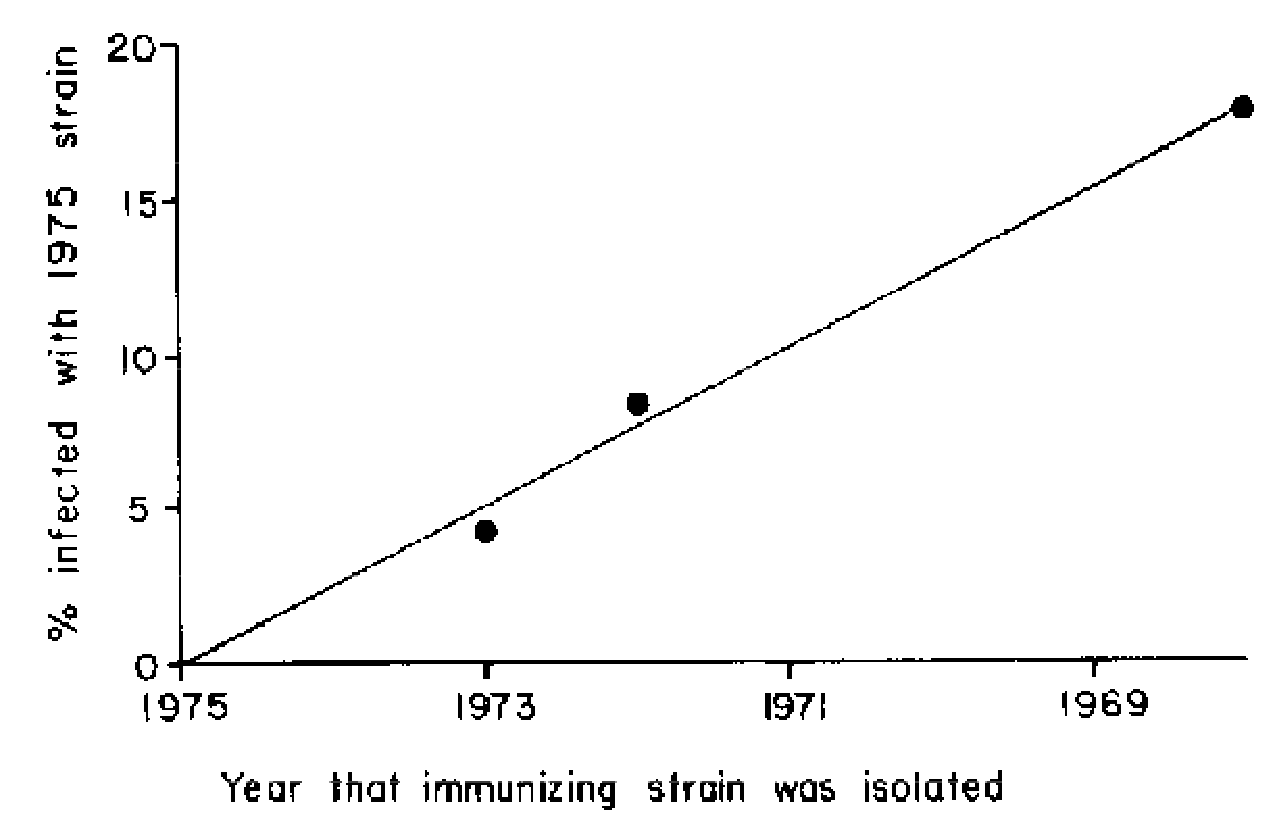
\includegraphics[width=0.5\linewidth]{graphs/intro/gill_murphy.eps}
  \end{center}
  \caption{Données de \citet{Gill1977} (reproduit d'aprés \citet{Pease1987})}
  \label{fig:intro:gill_murphy}
\end{figure}

L'expérience de \citet{Potter1977} permet de trancher entre ces
hypothèses. \citet{Potter1977} ont en effet immunisé des volontaires
avec différents vaccins dérivés de quatre souches de grippe A/H3N2
isolées en 1968, 1972, 1973 et 1974. Après 4 semaines, un temps
suffisamment court pour invalider l'hypothèse de la perte d'immunité,
ces volontaires ont été infectés par une souche virale de 1974. Les
résultats de cette expérience, présentés figure~\ref{fig:intro:potter}
montrent aussi une augmentation linéaire de la probabilité de
réinfection au fur et à mesure que le temps séparant les souches
immunisantes et le virus utilisé pour l'infection augmente. Cela
confirme l'hypothèse de l'augmentation du risque de réinfection du
fait de l'échappement des virus à l'immunité préexistante.

\begin{figure}[!htbp]
  \begin{center}
    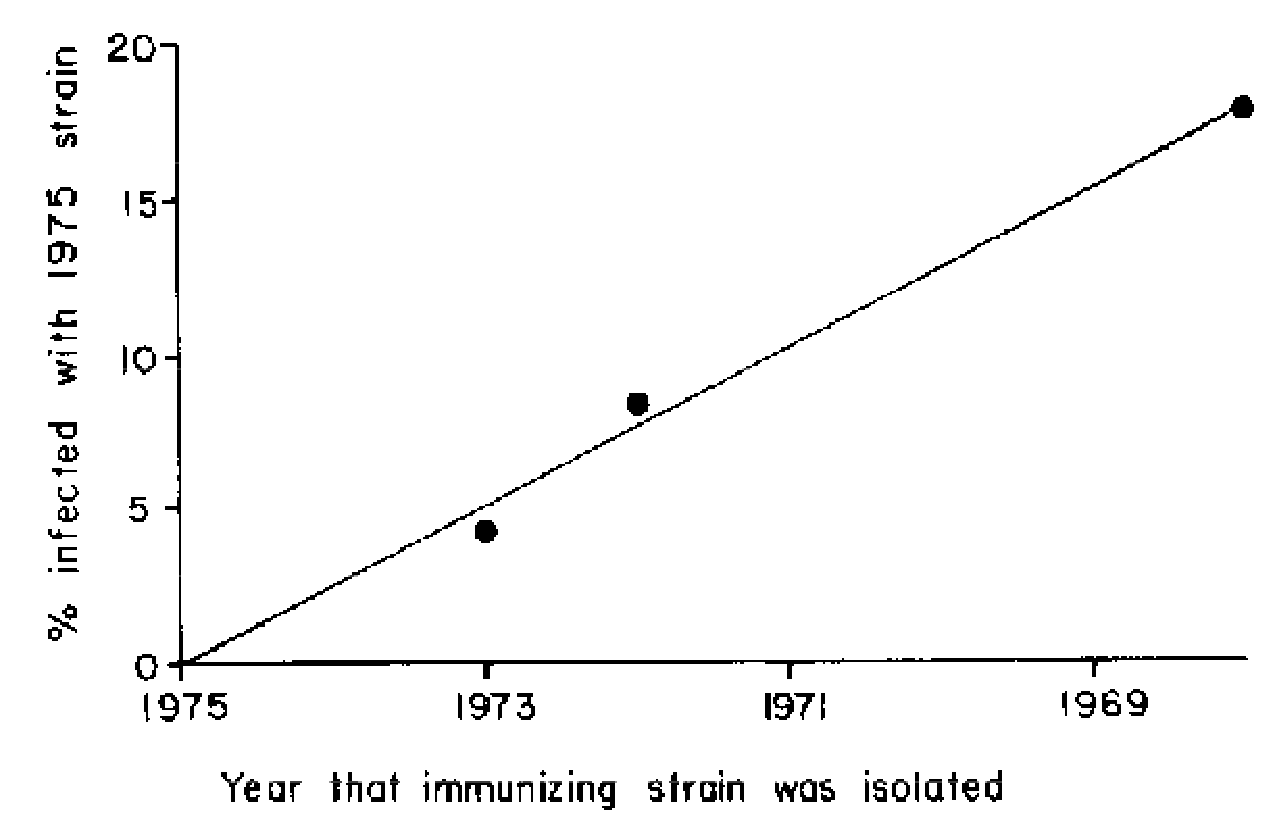
\includegraphics[width=0.5\linewidth]{graphs/intro/gill_murphy.eps}
  \end{center}
  \caption{Données de \citet{Potter1977} (reproduit d'aprés
    \citet{Pease1987})}
  \label{fig:intro:potter}
\end{figure}


Ce résultat permet à \citet{Pease1987} de proposer un nouveau modèle
pour les maladies récurrentes à évolution antigénique rapide.
Contrairement au paradigme classique des maladies infectieuses
infantiles où le renouveau des susceptibles se fait par les
naissances, dans le cas de la grippe ce renouveau de susceptibles se
fait par la perte d'immunité des hôtes du fait de l'évolution virale.
\citet{Pease1987} modélise alors l'évolution antigénique implicitement
par un changement de la susceptibilité des hôtes au cours du temps, en
accord avec les données disponibles à l'époque.

%\clearpage

\subsection{L'âge d'or de la génétique}

La révolution de la génétique des années 90 a permis l'acquisition
d'un nombre impressionnant de nouvelles données et une avancée majeure
dans la compréhension de l'évolution de la grippe A humaine. Les
années 90 ont donc vu les premières publications par \cite{Fitch1991}
et \citet{Fitch1997} de l'analyse phylogénétique des séquences du gène
HA1 (la région la plus immunogène de l'hemagglutinine).
\citet{Fitch1997} utilisent ainsi 254 séquences de HA1 obtenues de
1984 à 1996. Comme nous l'avons indiqué précédemment, cette étude a
révélé une diversité génétique relativement réduite à chaque instant
avec un arbre caractérisé par un tronc marqué comprenant de très
courtes branches. \citet{Fitch1997} ont ainsi montré que la durée
moyenne de survie des branches n'était que de 1.42 ans avec une durée
de 4.8 ans pour la branche la plus longue. Le nombre de substitutions
de nucléotides donnant lieu à des remplacements est 2.2 fois plus
élevé dans les branches que sur le tronc. Ce résultat peut s'expliquer
de différentes façons. On peut supposer que cet excès de mutations
dans les branches correspond à des mutations délétères (largement
majoritaires parmi les mutations) non encore purgées par la sélection
naturelle, et donc qui ne se retrouveront pas dans le tronc
ultérieurement. Cette hypothèse est intéressante, cependant en raison
des biais induits par le processus d'échantillonage et d'obtention des
séquences, elle ne peut être validée (nous verrons plus tard comment
les modèles multi-souches peuvent éclairer cette question). En effet
8\% des remplacements d'acides aminés observés sur HA1 peuvent être
attribués à des mutations liées à l'adaptation du virus aux oeufs
embryonnés utilisés pour les cultiver \citep{Bush2000}. Tout comme les
mutations délétères, les mutations produites par les oeufs ne se
retrouveront pas dans le tronc ultérieurement et peuvent donc ainsi
rendre compte de cette différence. Un second biais à même de rendre
compte de cette différence vient du fait que les données sont
fortement biaisées en faveur de variations antigéniques car
l'essentiel des séquences sont obtenues uniquement après un premier
tri visant à reconnaître les souches virales les plus divergentes d'un
point de vue antigénique dans le but de déterminer les futures
compositions vaccinales dans le cadre du programme de surveillance
globale de la grippe mis en place par l'OMS depuis 1952
\citep{Bush2000}. L'étude de \citet{Fitch1997} a aussi été le point de
départ d'une meilleure compréhension des processus sélectifs opérant
sur l'antigène principal de la grippe. La flexibilité de HA1 a été
mise en évidence en révélant que le nombre de substitutions de
nucléotides donnant lieu à des remplacement d'acides aminés était
distribué aléatoirement sur la position des codons (alors que
généralement on observe plus de substitutions conduisant à des
remplacements sur la première que sur la seconde position, les
substitutions étant plus conservatrices si elles ont lieu sur la
première position des codons). \citet{Fitch1997} et \citet{Bush1999}
ont aussi mis en évidence, en prenant garde de ne pas retenir de faux
positifs, 18 sites ou le ratio de substitutions non synonymes sur
synonymes était supérieur à 1, indiquant de la sélection positive.

\citet{Bush1999} ont cherché à comprendre dans quelle mesure les
codons sélectionnés positivement précédemment identifiés pouvaient
permettre de prédire l'évolution de la grippe A. Ces auteurs ont
montré que les lignées comportant le plus de mutations au niveau des
18 sites soumis à la sélection positive étaient pour 9 saisons sur 11
de 1986 à 1997 les lignées donnant naissance aux futures lignées
fructueuses engendrant le tronc de l'arbre. D'une manière remarquable,
si ces 18 codons sont associés à la région de reconnaissance des
anticorps, les codons de ces mêmes zones non soumis à la sélection
positive n'ont pas le même pouvoir prédictif, leur utilisation ne
permettant d'identifier les lignées fructueuses que dans 3 dans 11
saisons.
% predictabilité remise en question par la suite car les sites
% séléctioné changent !!!

L'accès à un nombre toujours grandissant de génomes complets
séquencés, accompagnés d'une augmentation conjointe de la puissance de
calcul nécessaire à leur analyse \citep{Holmes2007}, ont depuis permis
de nouvelles avancées dans ce domaine. Nous les détaillerons dans les
parties \ref{sec:intro:clusters}, \ref{sec:intro:sourcesink} et
\ref{sec:intro:debat} après avoir présenté les apports des modèles
mathématiques théoriques.


\subsection{Les modèles multi souches}

Du coté théorique, après les travaux de \citet{Pease1987}, de
nombreuses études ont cherché à modéliser explicitement les
différentes souches pour se rapprocher des analyses phylogénétiques.

L'approche la plus intuitive consiste peut-être à regrouper les hôtes
selon leurs histoires d'infections (approche $HB$ pour ``History
based'') comme introduit par \citet{Andreasen1997}. Ainsi, connaissant
l'histoire d'infection de chaque hôte, on peut établir des hypothèses
concernant l'effet du répertoire immunitaire acquis, face à une
infection par une nouvelle souche. Deux grandes catégories
d'hypothèses non mutuellement exclusives peuvent être faites. On peut
supposer:
\begin{itemize}
\item que l'immunité acquise suite aux infections précédentes confère
  une réduction de susceptibilité, limitant le risque de devenir
  infectieux ;
\item ou bien, que la protection partielle conférée par les infections
  précédentes se traduit par une moindre infectiosité suite à
  l'infection par la nouvelle souche (le risque d'infection étant le
  même que pour un hôte totalement naïf).
\end{itemize}

Il est alors naturel de supposer que la réduction de susceptibilité
($RS$) ou d'infectiosité ($RI$) est d'autant plus grande que les
souches nous ayant immunisé et allant nous infecter diffèrent
antigéniquement (immunité croisée). Lorsqu'un hôte immunisé par
plusieurs souches rencontre une souche n'appartenant pas à son
répertoire immunitaire, deux formulations sont principalement
utilisées pour décrire la protection partielle \citep{Gomes2002}:
\begin{itemize}
\item l'une suppose que l'immunité croisée agit de façon
  multiplicative, des anticorps de tout le répertoire immunitaire de
  l'hôte étant produits et leur action combinée étant supérieure à
  celle de chacun d'eux pris individuellement ;
\item et l'autre, que la protection partielle la plus forte détermine
  l'immunité croisée. Dans ce dernier cas, uniquement les anticorps du
  répertoire immunitaire de l'hôte les plus proches de la souche
  rencontrée sont produits.
\end{itemize}

Le principal obstacle à cette approche vient du fait de l'explosion du
nombre de variables d'états avec l'augmentation du nombre de souches.
Ainsi, pour une population comprenant $K$ souches, il y a $\sum_k
\binom{K}{k}=2^K$ histoires d'infections possibles. Comme le montre la
figure~\ref{fig:intro:multi}, passé $K=30$, ce nombre dépasse le
milliard. On ne peut donc pas espérer suivre la dynamique d'un grand
nombre de souches avec une telle approche, et, très rapidement, une
approche individu-centrée devient plus tractable.

\begin{figure}[!ht]
  \begin{center}
    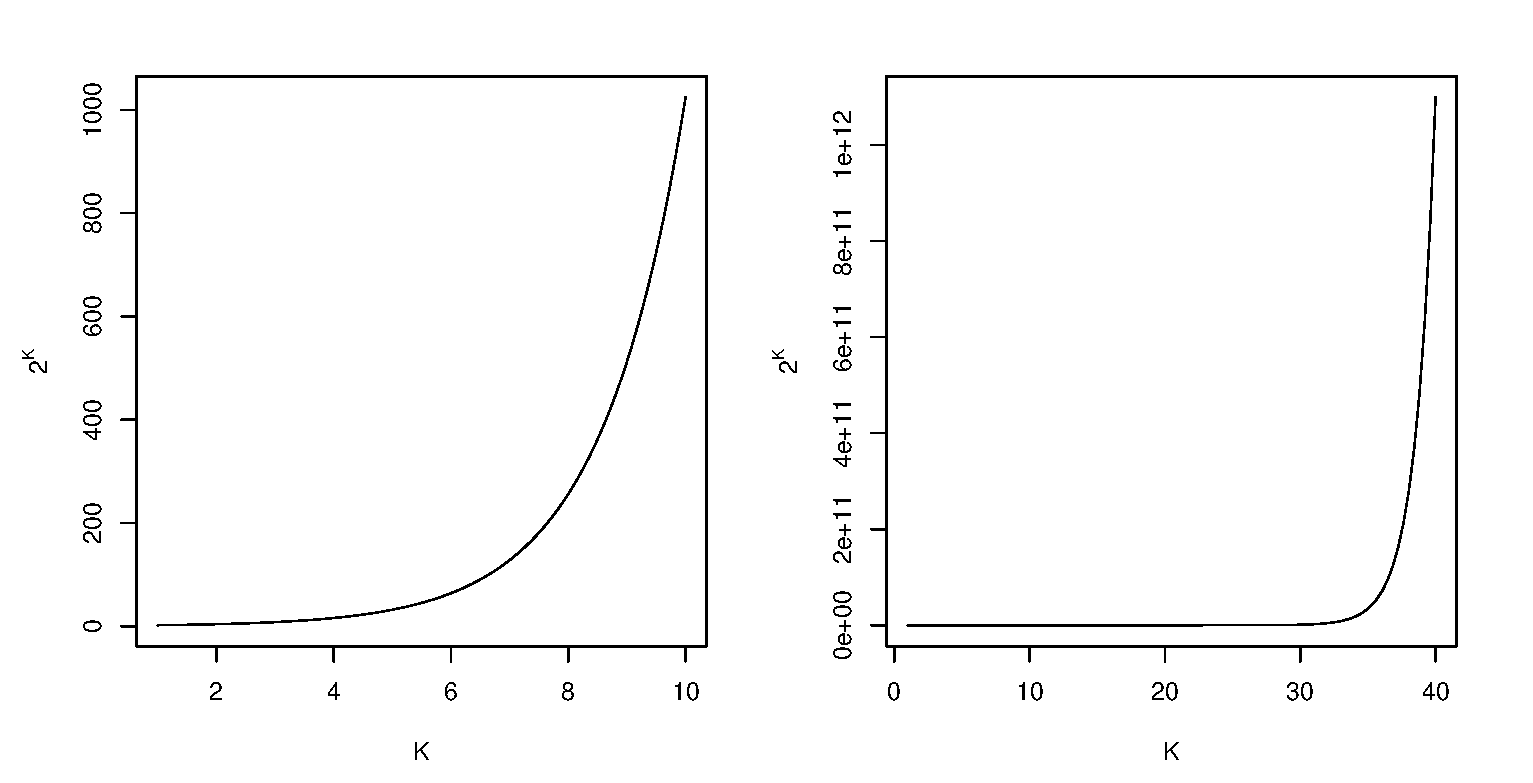
\includegraphics[width=0.8\linewidth]{graphs/R/multi.eps}
  \end{center}
  \caption{Augmentation du nombre de variables d'états en
    fonction du nombre de souches ($K$)}
  \label{fig:intro:multi}
\end{figure}

L'étude de la dynamique de système comprenant un petit nombre de
souches permet néanmoins de révéler des résultats intéressants comme
nous le montrerons par la suite (partie \ref{sec:intro:recyclage}).

Une autre approche des modèles multi-souches a été proposé par
\citet{Gog2002a}. Au lieu de suivre l'histoire infectieuse de la
population, ces auteurs ont proposé de suivre le statut immunologique
des hôtes en faisant l'hypothèse d'immunité croisée polarisée
(approche $SB$ pour ``status based''). Cette hypothèse suppose que le
statut immunologique est déterminé au moment de l'infection et résulte
immédiatement en l'acquisition d'une protection totale ou pas
(immunité polarisée) pour les souches antigéniquement voisines de la
souche infectante, selon des probabilités fonction de la distance
antigénique entre les souches. Considérons l'hypothèse $RS$ dans un
cas où il n'existe que 2 souches immunologiquement réactives (1 et 2)
pour mieux percevoir cette différence:
\begin{itemize}
\item Dans l'approche $HB$, l'infection par la souche 1 confère
  une protection partielle aux hôtes infectés ($R_1$). Cette
  protection ne s'applique que lors de la rencontre avec la souche
  2 antigéniquement proche et se matérialise par une probabilité
  réduite ($\sigma$) de devenir infecté par la souche 2. Si
  l'individu $R_1$ n'est pas infecté par la souche 2 lors de cette
  rencontre, il pourra l'être lors d'une rencontre ultérieure toujours
  avec la même probabilité réduite ($\sigma$).
\item Dans l'approche $SB$ le statut immunologique de notre hôte est
  déterminé au moment de l'infection par la souche 1. Selon une
  probabilité $\sigma'$, cet hôte acquiert une protection totale pour
  les souches 1 et 2 (devenant $R_{12}$).  Dans le cas
  complémentaire (probabilité $1-\sigma'$) il n'acquiert l'immunité
  que pour la souche 1 (devenant $R_1$) et reste donc totalement
  susceptible à la souche 2.
\end{itemize}

Les modèles $SB$ supposent aussi que l'immunité croisée agit de façon
multiplicative. En particulier, on suppose que les événements
d'acquisition d'immunité pour une souche $n$ lors d'une infection par
une souche $k$ (de probabilité $\sigma'_{kn}$) sont indépendants. On
peut ainsi calculer la probabilité $C(M,N,k)$ qu'un individu ayant un
statut immunologique $M$ acquiert un statut $N$, $M \subseteq N$,
suite à une infection par une souche $k$:

$C(M,N,k)$ =$
\begin{cases}
  \prod_{n \in N \setminus M} \sigma'_{kn} \prod_{n \notin N}
  (1-\sigma'_{kn}) & \text{si } k \notin M \text{ et } M \subset N \\
  0 & \text{sinon.}
\end{cases}$ 

où $N \setminus M$ dénote l'ensemble dont les éléments sont ceux de $N$ qui n'appartiennent pas à $M$. 


Une propriété remarquable de l'approche $SB$ a été mise en avant par
\citet{Gog2002}. Combiné à l'hypothèse $RI$ (et on autorisant la
coinfection), le formalisme basé sur le statut des hôtes permet de
réduire considérablement le nombre d'équations du système
multi-souches, en décrivant un système de $K$ souches avec exactement
$2K$ équations.

\citet{Gog2002} ont pu alors étudier comment différentes souches
immunologiquement réactives s'organisaient face à l'immunité
développée par une population d'hôtes. Ces auteurs ont considéré que
les souches évoluaient dans un espace unidimensionnel (une simple
ligne). Les souches pouvaient ainsi muter et donner naissance à des
souches filles voisines situées de part et d'autre de la souche
originelle. Un lien direct avec cet espace de souches permet de
modéliser l'immunité croisée, supposée décroître exponentiellement au
fur et à mesure que la distance entre les souches augmentent. Dans ce
contexte, \citet{Gog2002} révèlent que le système s'organise
différemment selon la durée de la période infectieuse des hôtes. Dans
le cas des maladies plutôt chroniques, différents clusters de souches
coexistent dans le temps, tandis que, pour des maladies à courte
période d'infection, des clusters de souches émergent et se remplacent
successivement au cours du temps. Ce dernier résultat n'est pas sans
rappeler les arbres phylogénétiques de HA1 précédemment décrits.
Ainsi, le système s'auto-organise, sous l'effet de l'immunité de la
population en groupe de souches aux propriétés antigéniques voisines.
\citet{Gog2002} montrent en particulier que leur modèle est en accord
avec l'hypothèse que les courtes branches latérales s'échappant du
tronc de l'arbre phylogénétique de HA1 pourraient être dues à des
souches ayant accumulé des mutations délétères, que nous avions énoncé
lors de la description des travaux de \citet{Fitch1997}. Pour ce
faire, ils utilisent un espace de souches bidimensionnel (un plan) où
la nouvelle dimension est associée à des mutations donnant lieu à des
virus moins transmissibles. Ils montrent alors que des virus
intrinsèquement moins transmissibles peuvent se maintenir un court
moment derrière les souches dominantes dont la progression engendre le
tronc d'un arbre. Le modèle de \citet{Gog2002} est donc remarquable
d'autant plus que l'aggrégation des souches en clusters antigéniques
sera montré empiriquement \citep{Plotkin2002, Smith2004}. Cependant
une des limitations de ces résultats est l'emploi d'un espace
antigénique de très faible dimension et donc très contraint.

\citet{Girvan2002} se sont intéressés à cette question en regardant
les conséquences de la dimensionalité de l'espace antigénique sur le
système multi-souches. Ces auteurs ont utilisé un modèle élégant
modélisant les séquences virales par des chaînes binaires. Dans ce
contexte, un espace antigénique de faible dimension peut être simulé
en supposant par exemple qu'à chaque mutation (représentée par le
changement d'un bit de 0 à 1) seul le bit le plus à gauche est muté.
Cela donne une évolution de la sorte:

\begin{verbatim}
00000000000000000
10000000000000000
11000000000000000
11100000000000000
\end{verbatim}

La distance antigénique est ensuite considérée en tenant compte du
nombre de différences entre les chaînes binaires présentes dans le
répertoire immunitaire de l'hôte et la souche infectante. Si la plus
petite de ces différences est supérieure à un seuil, l'hôte peut être
infecté, sinon, il est protégé.  \citet{Girvan2002} montrent que cet
espace antigénique contraint conduit à une diversité virale limitée et
produit des infections récurrentes en accord avec ce que l'on observe
pour la grippe.

La situation est par contre très différente lorsque l'on considère un
espace antigénique de grande dimension, obtenu par exemple en laissant
varier librement la position du bit mutant comme dans la séquence
ci-dessous:

\begin{verbatim}
00000000000000000
00000000010000000
00001000000000000
00000000010010000
\end{verbatim}

Dans ce cas, le nombre de souches ne cesse d'augmenter au cours du
temps, en désaccord avec les données phylogénétiques. Le modèle de
\citet{Girvan2002} incite donc à rechercher quels sont les facteurs
qui peuvent réduire le grand nombre de souches obtenu avec des modèles
considérant un espace antigénique réaliste de grande dimension.

\citet{Ferguson2003} s'attaquent à cette question dans un article
remarquable où ils considèrent un modèle individus centré, simulant
une population de 12 millions d'individus distribuée dans 20 patchs
géographiques où la transmission varie en opposition de phase dans
l'hemisphère Nord et Sud. Les souches sont caractérisées par
l'hémagglutinine et modélisées par 4 épitopes contenant chacun 3
codons. Ce système peut générer $4. 10^{15}$ souches. L'immunité
croisée varie en fonction d'une distance antigénique $d$ définie en
fonction du nombre de codons de la souche infectieuse n'ayant pas
d'acides aminés en commun avec ceux contenus dans le répertoire
immunitaire de l'hôte. \citet{Ferguson2003} suppose que l'immunité
croisée plafonne à une valeur élevée tant que $d$ est inférieur à 2
acides aminés puis qu'elle décroît linéairement jusqu'à une valeur
minimale.

Ces auteurs montrent d'abord que comme pour le modèle de
\citet{Girvan2002}, le système précédemment décrit conduit à une
explosion de la diversité de souches et une prévalence excessive. Ce
résultat est en particulier robuste à l'inclusion de contraintes
fonctionnelles. Cette explosion de diversité virale se comprend assez
bien étant donné que l'immunité croisée décroît avec la distance
antigénique. Ainsi, lorsque la diversité antigénique augmente, la
prévalence augmente aussi et cela renforce la production d'autres
variants. \citet{Ferguson2003} postulent alors l'existence d'un
processus de densité dépendance agissant à l'échelle de temps de
l'apparition des souches pour expliquer la réduction de la diversité
virale. Ces auteurs suggèrent que ce processus pourrait être le fait
d'une période temporaire de courte durée d'immunité totale (protégeant
contre toutes les souches et tous les sous-types de grippe) due à
l'action des lymphocyte T cytotoxique (CD8 +T) dirigée contre les
protéines internes du virus fortement conservées. L'importance de
cette composante de la réponse immunitaire avait été soulignée par
ailleurs par \citet{Webster1992} comme un des facteurs pouvant
expliquer le remplacement des sous-types grippaux lors des précédentes
pandémies dans un contexte où l'immunité croisée entre les sous-types
est présumée être faible. Les lymphocytes CD8 +T sont considérés
importants pour la guérison d'une infection grippale mais ne sont
généralement pas suffisants pour protéger contre les réinfections
ultérieures en l'absence d'anticorps. En effet, leur quantité diminue
trop rapidement après la première infection pour rester effective et
le temps nécessaire à leur rappel est trop élevé pour empêcher
l'établissement d'un nouveau virus \citep{Grebe2008}.

\citet{Ferguson2003} montrent que l'inclusion de cette période
temporaire d'immunité totale (les auteurs la prennent égale à 6 mois)
suffit à réduire la diversité virale, et permet d'obtenir des
phylogénies identiques à celles obtenues pour HA de H3N2. Ils montrent
en outre que la réduction du taux de mutation et de l'intensité de
l'immunité croisée permet d'obtenir des phylogénies avec plusieurs
lignées co-circulantes, comme c'est le cas pour la grippe B et dans
une moindre mesure H1N1, la valeur de $R_0$ n'ayant que peu
d'influence. Les auteurs confirment les prédictions de
\citet{Webster1992} et montrent que la période d'immunité croisée est
cruciale pour obtenir des remplacements de sous-types lors des
pandémies. Ils parviennent aussi à reproduire le cas de la
réintroduction de H1N1 en 1977 qui mène à la coexistence avec H3N2.

Le modèle de \citet{Ferguson2003} est séduisant sous bien des aspects,
cependant sa complexité rend son étude difficile. En particulier, il
est difficile de bien caractériser les chaînes causales menant aux
dynamiques observées. \citet{Tria2005} ont donc proposé de regarder
quels sont les facteurs minimaux pouvant expliquer les résultats de
\citet{Ferguson2003}. Pour ce faire ils ont considéré un modèle proche
de celui de \citet{Girvan2002} et négligé tous les processus spatiaux
inclus dans le modèle de \citet{Ferguson2003}. \citet{Tria2005}
partent d'un modèle de base ne comportant que de l'immunité croisée et
montrent que la présence additionnelle de la seule période d'immunité
temporaire totale ne suffit pas à réduire la diversité virale. Pour
retrouver un nombre de souches réduit, cette période de protection
totale doit être accompagnée d'une forme d'hétérogénéité.
\citet{Tria2005} l'incluent en supposant que les mutants ont des taux
de transmission variables tirés dans une loi Gamma. Ils supposent que
cette hétérogénéité est aussi présente dans le modèle de
\citet{Ferguson2003} par l'intermédiaire de la dynamique spatiale.

Cependant, une différence importante existe dans la façon dont
\citet{Ferguson2003} et \citet{Tria2005} ont modélisé la période
temporaire d'immunité croisée. \citet{Tria2005} ont simplement supposé
qu'une fois guéris, les hôtes restaient un temps défini
``invincible'', tandis que \citet{Ferguson2003} ont considéré en plus
que toutes les expositions ne donnant pas lieu à une infection étaient
suivies d'un ``boosting'' de la période d'invincibilité (alors étendue
de sa durée moyenne) sans mise à jour du répertoire immunitaire. Les
auteurs justifient ce processus par l'existence du péché antigénique
originel (\citet{Francis1953}, \citet{St1966}, \citet{St1966a} ou
\citet{Kim2009} pour une synthèse récente) qui établit que lors
d'infections séquentielles, la réponse immunitaire cible
préférentiellement les antigènes de la souche rencontrés initialement
plutôt que les antigènes mutés de nouvelles souches antigeniquement
proches, permettant à ces nouveaux virus d'échapper en grande partie à
la réponse immunitaire.  Notons que le péché antigénique originel
justifie le fait de ne pas mettre à jour le répertoire immunitaire des
expositions à des souches antigéniquement proche ne donnant pas lieu à
des infections mais il ne justifie pas nécessairement de ``booster''
la période d'invincibilité des hôtes rencontrant des souches pour
lesquelles ils sont déjà immunisés et ne redeviennent pas infectieux.
Ce ``boosting'' additionnel est reporté comme une contrainte densité
dépendante importante réduisant la diversité virale, l'incidence et
les taux de fixation dans les annexes de leur papier et nous supposons
que cette différence majeure peut être à l'origine des résultats
rapportés par \citet{Tria2005}.

\citet{Minayev2008, Minayev2009} ont proposé un modèle analytique
cherchant à se rapprocher du modèle de \citet{Ferguson2003}. Ils ont
donc mis de côté l'approche $SB$ impliquant une immunité croisée
multiplicative et ont privilégié le formalisme $HB$.  Leur modèle est
basé sur celui de \citet{Gupta1998} qui ont montré qu'en décrivant les
souches par un système génétique de $L$ loci comprenant $A$ allèles,
on pouvait obtenir un système dont le nombre d'équations augmente
linéairement avec le nombre de souches (donné par $A^L$) à condition:
\begin{itemize}
\item d'utiliser des variables d'états se recoupant,
\item de permettre la coinfection,
\item et de considérer une forme spéciale de l'hypothèse de
réduction d'infectiosité décrite ci-dessous. 
\end{itemize}
Dans le modèle de \citet{Gupta1998}, les hôtes partiellement protégés
sont tous totalement susceptibles à une souche immunologiquement
réactive, mais suite à l'infection, seulement une partie des hôtes
infectés deviennent infectieux, la partie complémentaire acquérant une
immunité pour la souche rencontrée sans devenir infectieux.  Dans sa
version originale, ce modèle ne prévoyait qu'un seul niveau d'immunité
croisée selon que les souches aient un allèle en commun ou pas.
\citet{Minayev2008} ont généralisé ce modèle pour prendre en compte
différents niveaux d'immunité croisée (en supposant que la protection
croisée soit définie par le nombre d'alléles en commun des souches)
tout en gardant un nombre d'équations augmentant linéairement avec le
nombre de souches. Ce modèle, sans doute le plus tractable dans les
approches $HB$ comporte au final ``seulement'' $A^L(L+1)$ équations.

\citet{Minayev2008, Minayev2009} confirment alors l'explosion de la
diversité virale en l'absence de période d'immunité totale temporaire.
Ces auteurs veulent ensuite étudier l'effet de la période
d'invincibilité (en l'introduisant tout comme \citet{Ferguson2003} et
donc en considérant un ``boosting'' de la période d'invincibilité sans
mise à jour du répertoire immunitaire suite aux expositions ne donnant
pas lieu à des infections). Leurs résultats sont dans ce cas à prendre
avec précaution car les équations introduisant la période
d'invincibilité temporaire sont inconsistantes.  Brièvement,
l'équation (4.2) de \citet{Minayev2008} (respectivement équation (2.6)
dans \citep{Minayev2009}) stipule que les infections peuvent provenir
d'une souche déjà présente dans le répertoire immunitaire et que dans
ce cas, les hôtes ne deviennent pas infectieux mais développent une
invincibilité de 6 mois.  Cependant, les auteurs précisent aussi que
l'équation (2.1) des 2 papiers reste identique ce qui est en
contradiction avec l'équation (4.2) (respectivement (2.6)) étant donné
le fait que l'équation (2.1) implique que les hôtes ne peuvent pas
être infectés ou développer une immunité totale temporaire s'ils sont
exposés à des souches déjà présentes dans leur répertoire
immunitaire. Il faudrait donc revisiter les parties de ces papiers
impliquant la période d'immunité totale temporaire avant d'en tirer
des conclusions.

%\clearpage

\subsection{Les clusters antigéniques}
\label{sec:intro:clusters}

Du coté des donnés, \citet{Plotkin2002} ont utilisé une approche
complémentaire à la reconstruction phylogénétique en regardant s'il
existait une unité naturelle d'agrégation des différentes souches.
\citet{Plotkin2002} ont ainsi montré que l'on pouvait regrouper
différentes souches en clusters en considérant par exemple comme
critère de regroupement le nombre d'acides aminés différents (distance
de Hamming). Les clusters, définis à partir de 560 séquences du gène
codant pour la région HA1 de l'HA de H3N2 échantillonné entre 1968 et
2000, apparaissent se succéder au cour du temps et se remplacent tous
les 2-5 ans, rappelant les résultats obtenus par \citet{Gog2002}. Ces
clusters, définis uniquement à partir de la séquence d'acides aminés,
se trouvent être en plus de bons prédicteurs de la propriété
antigénique des virus sous-jacents. En particulier, en utilisant la
souche la plus récente du cluster dominant d'une saison de grippe
donnée, \citet{Plotkin2002} obtiennent des recommandations vaccinales
identiques à celles de l'OMS, basées sur la caractérisation des
propriétés antigéniques des souches, pour 9 des 16 saisons
considérées. Ces auteurs révèlent des relations intéressantes entre la
variation des acides aminés au cours du temps pour les 5 épitopes
majeurs de HA1 aussi bien au sein qu'entre les clusters. Il apparaît
en particulier, que chaque changement de cluster est principalement le
résultat d'une forte variation au sein d'un épitope, lui-même
différent de l'épitope le plus variable lors du précédent changement
de cluster. Enfin, une forte corrélation est reportée entre la
variation d'acides aminés intra cluster et la distance selon la
métrique de Haming entre les différents clusters. Tout se passe donc
comme si les changements entre clusters n'étaient possibles que
lorsque la sélection naturelle a suffisamment de variabilité au sein
d'un cluster pour s'exprimer.

La mise en avant des clusters comme unité de base sur laquelle fonder
un raisonnement évolutif par \citet{Plotkin2002} a été largement
confirmée et précisée par les travaux de \citet{Smith2004}.
\citet{Smith2004} se sont intéressés au lien qu'il y avait entre
génotype et phénotype (en particulier la propriété antigénique).
L'inférence des propriétés antigéniques des HA des différentes souches
est réalisée par le test d'inhibition de l'hemagglutination (HI)
\citep{Miller1944}. Ce test repose sur la capacité de l'HA des virus
grippaux à agglutiner des globules rouges et à la capacité de sérum
animaux produits par réaction aux différents virus grippaux à inhiber
cette agglutination (plus ou moins bien en fonction de la distance
antigénique séparant les virus). Cette technique est utilisée de
manière standard par l'OMS pour établir les compositions vaccinales.
En particulier, il est considéré qu'une dilution de facteur 4 du sérum
lors du test HI impose de mettre à jour le vaccin. Utilisant une
approche multivariée, \citet{Smith2004} ont pu révéler les relations
antigéniques de 273 isolats (dont 94 proviennent de Hollande, les
autres du reste du monde) prélevés entre 1968 et 2003 soumis à des
test HI croisés. Ces auteurs montrent ainsi que s'il existe une
correspondance remarquable entre l'évolution génétique et antigénique
des virus, des différences significatives existent. Si l'évolution
génétique du virus est largement graduelle, l'évolution antigénique
est elle ponctuée. Les différentes souches s'organisent en clusters
présentant des propriétés antigéniques semblables, et les clusters
restent dominant entre 1 et 8 saisons avec une moyenne 3.3 ans ($\pm
1.9$) avant d'être remplacés. En particulier, l'évolution antigénique
s'opère principalement dans un espace à 2 dimensions dans lequel les
clusters s'organisent chronologiquement selon un axe majoritaire
accompagné de variations ``en zigzag'' dans l'autre dimension
(figure~\ref{fig:intro:smith}).  Les transitions de clusters sont le
fait d'un nombre variable de changements d'acides aminés. Le
changement d'un seul acide aminé peut suffire à précipiter un
changement de cluster. C'est par exemple le cas de la mutation N145K
liée à la transition du cluster SI87 à BE89 et BE92 à WU95. Les
changements d'acides aminés corrélés aux changements de clusters
antigéniques correspondent à l'étude des codons sous sélection
positive par \citet{Bush1999} uniquement pour la période 1985-1997
correspondant aux séquences de cette dernière étude.  L'absence de
correspondance pour les autres périodes temporelles va de pair avec
l'hypothèse d'un changement des sites sélectionnés au cours du temps
déja révélé par \citet{Plotkin2002} et posant des limites à la
possibilité de prédire l'évolution de HA1 comme l'avait laissé
entrevoir l'étude de \citet{Bush1999}.

\begin{figure}[!htbp]
  \begin{center}
    \includegraphics[width=0.5\linewidth]{graphs/intro/smith.eps}
  \end{center}
  \caption{Cartographie antigénique des virus A/H3N2 isolé de 1968 à
    2003. (reproduit d'après \citet{Smith2004}).}
  \label{fig:intro:smith}
\end{figure}


\citet{Blackburne2008} se sont intéressés à cette question en
comparant différents modèles d'évolution moléculaire d'une complexité
croissante pouvant être sélectionnés par AIC ou ratio de vraisemblance.
En utilisant les même données que \citet{Smith2004} (254 séquences
isolées de 1968 à 2003) ces auteurs montrent que le modèle le plus
adapté pour rendre compte des données comporte un ensemble de matrices
de substitutions différentes pour différentes régions de la protéine
et où le taux de substitution peut changer au cours du temps,
correspondant à un changement de pressions de sélection.
\citet{Blackburne2008} valident ainsi l'hypothèse que les sites de HA1
soumis à la sélection positive varient au cours du temps, rendant la
distinction entre site antigénique et non antigénique plus subtile et
labile que précédemment considérée. En particulier, ces auteurs
montrent que beaucoup de changements de pressions de sélection ont
lieu au niveau de sites non directement associés au changement
d'acides aminés menant à des transitions de clusters antigéniques. Ces
mutations peuvent être impliquées dans le maintien de la
fonctionnalité de HA (potentiellement mise à mal par les autres
changements ayant conduit à des modifications des propriétés
antigéniques), ou bien encore, peuvent assurer la stabilité
thermodynamique de la macromolécule.

Du coté théorique, \citet{Koelle2006} ont montré que le caractère
ponctué de l'évolution antigénique de HA de la grippe A/H3N2 se
révélait être primordiale dans la détermination de la phylodynamique
du virus.  Influencés par le papier de \citet{Smith2004},
\citet{Koelle2006} se sont en particulier intéressé au lien qu'il
existe entre génotype et phénotype de HA. Là où les approches
précédentes avaient considéré un lien linéaire entre séquence
génétique et propriété antigénique, \citet{Koelle2006} ont modélisé ce
lien explicitement par un modèle de réseau neutre pour protéine
appliqué à HA. Schématiquement ce modèle suppose l'existence de
périodes où la structure de l'antigène varie peu, dû au fait que les
mutations sont principalement des mutations neutres ou quasi neutres
(peu d'influence sur la stucture tridimensionnelle de la protéine),
tandis que ponctuellement, de rares mutations peuvent précipiter un
changement de structure tridimensionnelle de l'antigène (et donc
grandement changer les propriétés antigéniques). Ce modèle prend en
compte les interactions complexes entre les différents acides aminés
des épitopes et accorde une importance au contexte dans lequel chaque
mutation apparaît. La considération d'un lien non linéaire et dégénéré
entre génotype et phénotype permet une interprétation aisée des
clusters antigéniques mis en évidence par \citet{Smith2004}.  En
particulier, il permet de rendre compte du fait que certaines
transitions de clusters sont le fait d'une seule mutation
(apparaissant dans un contexte particulier) tandis que certains
clusters gardent une même propriété antigénique tout en arborant une
grande variété de souches (par exemple 2 souches du cluster HK68
diffèrent de 19 acides aminés). Le modèle de réseau neutre pour HA est
aussi consistant avec la mise en évidence par \citet{Plotkin2002} d'un
lien entre l'accumulation de diversité d'acides aminés au sein d'un
cluster et le changement de cluster.

Au niveau épidémiologique, \citet{Koelle2006} modélise alors la
dynamique des clusters antigéniques du sous-type H3N2 en se focalisant
sur le niveau du phénotype. Par souci de simplicité,
\citet{Koelle2006} utilisent le modèle de \citet{Gog2002} (approche
$SB$ et hypothèse $RI$) et rajoutent un terme de forçage saisonnier
pour s'intéresser aux régions tempérées d'où proviennent l'essentiel
des données. Les auteurs sont obligés de prendre en compte une
structure spatiale implicite faisant intervenir une forte immigration
pour compenser les extinctions observées pendant la période
inter-épidémique. Partant de cette base, \citet{Koelle2006} montrent
que leur modèle permet d'obtenir des dynamiques très proches de celles
observées dans les zones tempérées. En particulier, le modèle prédit
une augmentation de la diversité virale jusqu'à ce qu'un nouveau
cluster antigénique apparaisse et que, du fait de son échappement à
l'immunité de la population, il soit suffisamment avantagé pour
remplacer le cluster précédent dans un balayage sélectif. Ainsi, la
diversité virale reste limitée dans le temps, et le modèle reproduit
la succession de clusters antigéniques observés. Au niveau
épidémiologique, les transitions de cluster s'accompagnent
généralement d'une épidémie plus marquée, souvent suivie d'une période
réfractaire (faible épidémie de H3N2) la saison suivante.
\citet{Koelle2006} remarquent que cette tendance est présente dans les
données des USA avec une période réfractaire observée pour 6 des 7
changements de clusters postérieurs à HK68. D'une manière remarquable,
dans 6 de ces 7 périodes réfractaires potentielles, H1N1 ou la grippe
B domine.

Le modèle de \citet{Koelle2006} illustre donc que la prise en compte
de l'évolution ponctuée de HA et donc l'échappement ponctué à
l'immunité de la population par la grippe suffit à rendre compte des
principales caractéristiques de H3N2. En particulier, la présence
d'une période d'immunité totale temporaire n'est pas nécessaire pour
expliquer la diversité génétique réduite observée dans les
phylogénies.  Par ailleurs, \citet{Koelle2006} rapportent que des
valeurs de $R_0$ plus faibles que celles utilisées pour leurs
simulations de H3N2 ($R_0 =5$) induisent des dynamiques durant
lesquelles des clusters antigéniques coexistent et les phylogénies
présentent plus de branchements, en accord avec ce que l'on observe
pour H1N1 et la grippe B.


Indépendemment des réseaux neutres, le modèle de \citet{Koelle2006}
met en évidence l'importance potentielle des balayages sélectifs et
des dynamiques transitoires comme éléments clefs pour comprendre la
phylodynamique de la grippe. Cette idée maîtresse peut donc aussi
s'appliquer lors des réassortiments intra-sous-type pouvant être
considérés dans certains cas à l'échelle du phénotype comme de rares
``mutations'' ayant de grands effets antigéniques. Les analyses de
génomes entiers, font en effet de plus en plus apparaître les
réassortiments intra-sous-type comme des évènements évolutifs
important pour la grippe \citep{Holmes2005, Nelson2007}. Par exemple,
dans une étude phylogénétique de 156 génomes complets de H3N2
collectés dans l'état de New York entre 1999 et 2004,
\citet{Holmes2005} ont montré que l'origine du cluster antgénique FU02
était dû à un réassortiment intra-sous-type entre différentes lignées
co-circulant de H3N2.  Cependant les exemples les plus marquants sont
peut-être ceux concernant H1N1. Au niveau épidémiologique, les
épidémies de 1947 et 1951 sont particulièrement marquantes. En 1947,
le vaccin alors efficace les années précédentes est un échec total et
les souches grippales apparaissent tellement différentes de celles des
années antérieures que la littérature de l'époque parle d'une nouvelle
famille de virus (A', par opposition à A les années précédentes).
\citet{Kilbourne2002} reviennent sur cette épidémie et montrent que
les HA des souches des familles A et A' n'ont que 5\% de réactivité
antigénique. Pour l'épidémie de 1951, \citet{Viboud2006b} montrent que
son impact en termes de mortalité et sa transmissibilité sont plus
élevés que lors des pandémies de 1957 et 1968 au Royaume unis et au
Canada. Une partie des causes de ces épidémies particulières ont été
révélées par l'analyse de \citet{Nelson2008}. Les auteurs ont analysé
71 génomes complets de H1N1 échantillonnés entre 1918 et 2006. Ils
montrent que l'épidémie de 1947 est liée à un réassortiment intra
sous-types permettant au virus prédominant de 1943 à 1945 d'acquérir
de nouveaux fragments d'ARN codant pour PB2, PA, HA, NP et NS
provenant vraisemblablement d'une lignée de H1N1 minoritaires et non
mise en évidence lors de la surveillance de l'époque. Le changement de
HA explique ainsi la forte divergence antigénique de la souche de
1947. Pour 1951, la même étude révèle que cette épidémie est
probablement liée à un réassortiment où les souches prédominantes
auraient gardé le même fragment d'ARN pour HA, mais acquis deux
nouveaux gènes codant pour les polymerases PB1 et PA.

Ces résultats montrent l'importance des réassortiments intra-sous-type
mais permettent aussi de tempérer un peu la vision simplifiée offerte
par la théorie de l'échappement ponctué à l'immunité. En effet, les
épidémies de 1947 et 1951 nous rappellent que la variation de HA n'est
pas toujours le déterminant majeur gouvernant la taille des épidémies.
L'épidémie de 1951, où à priori les deux antigènes principaux (HA et
NA) n'ont pas changé, a en effet été plus sévère que celle de 1947 où
un HA radicalement différent des précédents a émergé. Les interactions
entre les différents fragments du génome sont donc essentiels à
prendre en considération si l'on veut bien appréhender les
conséquences de l'évolution virale sur les dynamiques épidémiologiques
et la rétroaction qui s'en suit. Nous rediscuterons de ce point de
manière détaillée par la suite (partie \ref{sec:intro:sourcesink}).

Pour conclure cette section, il est intéressant de constater que le
changement de paradigme concernant l'évolution antigénique de la
grippe A permet de concilier deux hypothèses débattues dans les années
1950 et 1960, illustrées par les figures~\ref{fig:intro:francis1}
et~\ref{fig:intro:francis2}.

\begin{figure}[!htbp]
  \begin{center}
    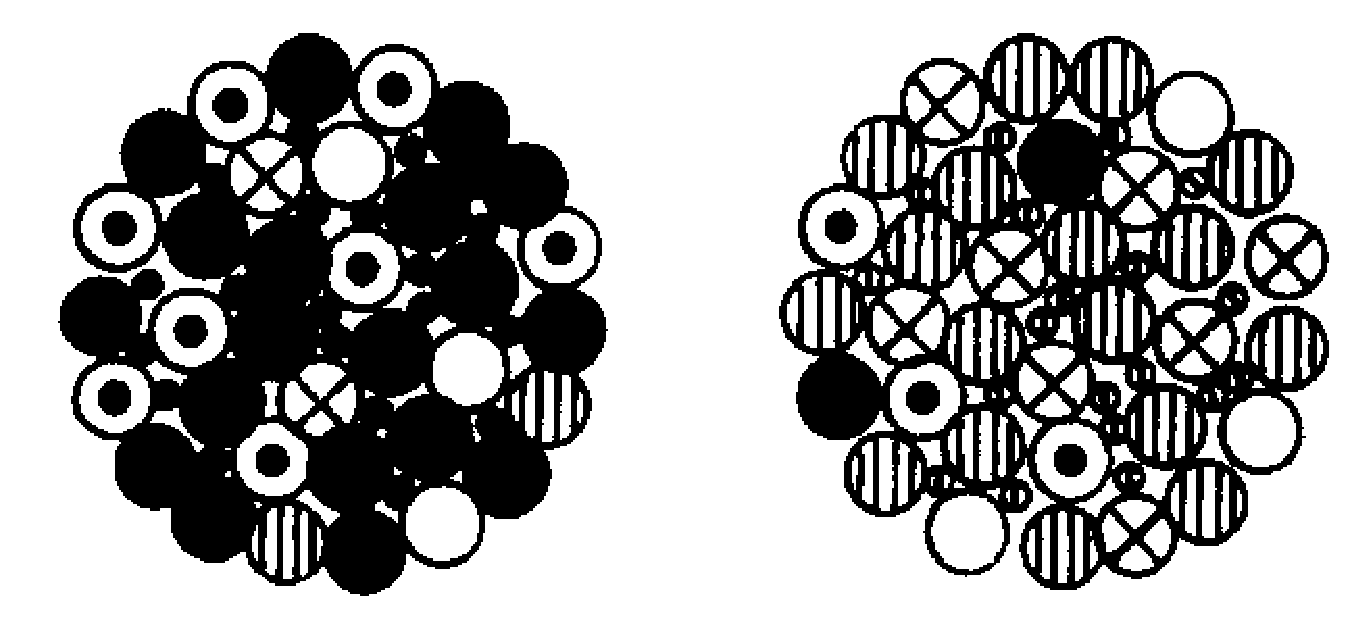
\includegraphics[width=0.5\linewidth]{graphs/intro/francis1.eps}
  \end{center}
  \caption{Illustration de l'hypothèse selon laquelle les variations
    antigéniques de la grippes sont le fait de rearangements d'un
    nombre fini d'antigènes (reproduit d'après \citet{Francis1960}).}
  \label{fig:intro:francis1}
\end{figure}

\begin{figure}[!htbp]
  \begin{center}
    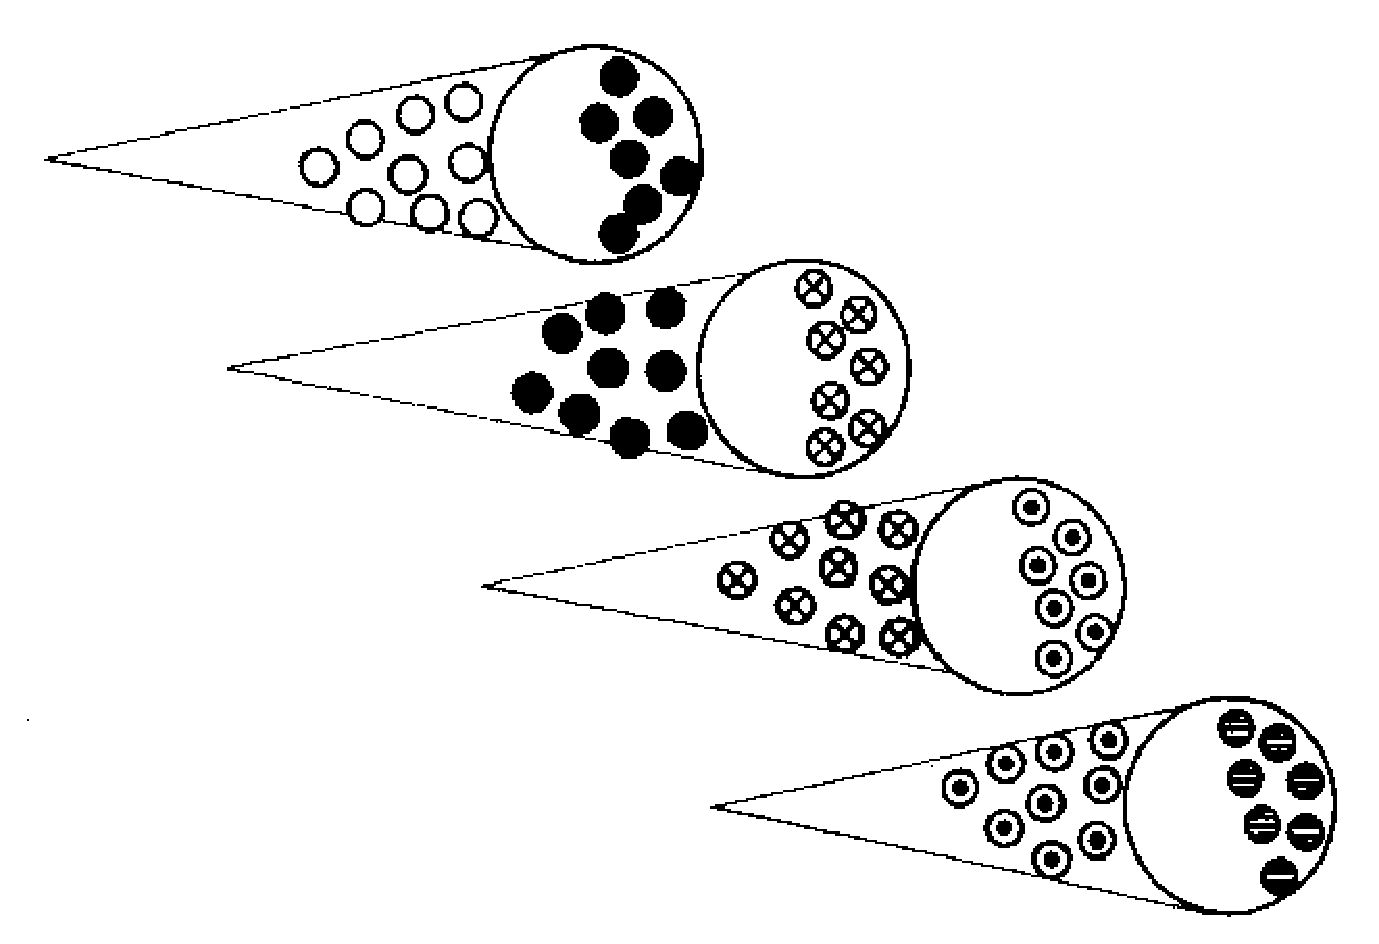
\includegraphics[width=0.5\linewidth]{graphs/intro/francis2.eps}
  \end{center}
  \caption{Illustration de l'hypothèse de la perte et gain d'antigènes
    pour les variants successifs de grippes (reproduit d'après
    \citet{Francis1960}).}
  \label{fig:intro:francis2}
\end{figure}

Les interrogations portaient sur la nature des changement antigéniques
des virus avec en confrontation, une vision selon laquelle ces
changements étaient le fait de ré-arrangement de différent antigènes
présents en un nombre fini, face à une vision où les changements
antigéniques résultaient du remplacement de différents antigènes au
cour du temps \citep{Francis1960}.

L'étude de \citet{Jensen1957} entre autre, avait permis d'opter pour
la première de ces hypothèses (figure~\ref{fig:intro:francis1}).  Les
auteurs ont caractérisé les propriétés antigéniques des variants de
H1N1 des familles A de 1933 à 1944 et A' de 1946 à 1955.  Pour ce
faire, ils ont établi un indice de réaction pour chaque souche défini
comme le nombre de souches avec lesquelles la souche étudiée interagit
fortement. Ainsi, une souche antigéniquement identique à toutes les
souches d'une série de 28 aura un indice de 28. Avec cette mesure, si
de nouveaux antigènes ne cessent d'apparaître au cours du temps, on
s'attend à observer une évolution croissante des indices. Si par
contre le nombre d'antigènes diminue, les indices devraient décroître
au cours du temps. Enfin, dans le cas où les antigènes se remplacent,
ont devrait avoir une courbe en cloche avec un maximum à mi-temps pour
les 2 familles. \citet{Jensen1957} révèlent que la distribution des
indices au sein de chaque famille (A et A') ne suit aucune de ces
évolutions. Les indices varient bien, indiquant une variabilité
antigénique mais sans tendance particulière au cours du temps.

Les résultats de \citet{Koelle2006} et, \citet{Blackburne2008}
permettent d'unifier ces deux hypothèses en attribuant la première à
des changements antigéniques intra-cluster et la seconde aux
transitions entre les clusters suivies de balayages sélectifs et de
changements de sites soumis à la sélection positive.

%\clearpage

\subsection{Une évolution antigénique graduelle ou ponctuée ?}
\label{sec:intro:debat}

\citet{Wolf2006} ont fourni une confirmation du changement de
perspective majeure dans l'appréhension de la dérive antigénique de la
grippe.  Ces auteurs ont utilisé plus de 1000 génomes complets
séquencés obtenus entre 1995 et 2005 pour les grippes A/H3N2 et
A/H1N1. Contrairement aux analyses précédentes, ces prélèvements ne
sont pas biaisés en faveur de la variation antigénique offrant la
garantie d'un meilleur reflet des différences de fitness entre les
lignées.  En accord avec les études antérieures, \citet{Wolf2006} ont
mis en évidence de la sélection positive (avec un ratio de
substitutions non synonymes sur synonymes supérieur à 1) pour les
sites situés au niveau du tronc de l'arbre appartenant à la région des
épitopes de HA.  Aucune trace de sélection positive n'a été détectée
en dehors de ces régions.  Le résultat n'apparaît cependant pas
statistiquement significatif, très probablement en raison du nombre
trop restreint de mutations sur le tronc de l'arbre pour avoir une
puissance suffisante. \citet{Wolf2006} ont ensuite cherché des
signatures de la sélection positive en considérant les temps
d'extinction des différentes lignées, définies arbitrairement à chaque
point de branchement de l'arbre phylogénétique pour la région de
HA. Les auteurs ont trouvé que la distribution des temps d'extinction
était bimodale avec des lignées caractérisées par de courts temps
d'extinction (inférieur à 6 mois), et d'autres, marquées par un temps
d'extinction beaucoup plus lent (supérieur à 6 mois). Dans ce
contexte, des temps d'extinctions courts sont à relier à un
remplacement rapide des nouvelles lignées, ce qui va dans le sens d'un
avantage sélectif pour les lignées capables de remplacer rapidement
leur prédécesseur. Cette idée est renforcée par la présence d'un excès
significatif de substitutions non synonymes pour les sites des
épitopes situés dans les régions du tronc caractérisées par des temps
d'extinctions rapides. Ces résultats amènent \citet{Wolf2006} à
conclure que l'essentiel de la sélection positive à lieu pendant de
courtes périodes (matérialisées par les régions du tronc associées à
des remplacements de lignées rapides) entre lesquelles se déroulent
des périodes plus longues de stase évolutive (matérialisées par les
régions du tronc ou les temps d'extinctions des lignées sont
lents). Par ailleurs, la présence de nombreuses mutations identiques
ayant lieu dans des lignées multiples majoritairement pendant ces
``bursts'' de sélection positive laisse à penser que le nombre de
trajectoires évolutives possible est limité.

\citet{Wolf2006} se sont aussi intéressés aux conséquences
épidémiologiques de leurs résultats. En particulier, n'ayant pas
détecté de traces de séléction positive pour HA de H1N1, ces auteurs
ont proposé que la dominance de H1N1 pendant certaines saisons de
grippes pouvait être due au fait d'une diminution de fitness relative
de H3N2, résultant d'une déplétion de la population d'hôtes
susceptibles à H3N2 non renouvelée durant les intervalles de stase
évolutive de ce sous-types. \citet{Wolf2006} rapportent ainsi qu'aux
Etats-Unis, les saisons de H3N2 précédent H1N1 sont caractérisées par
une diffusion significativement plus lente et un impact tendant a être
plus faible en terme de mortalité. L'accord de ces résultats avec
l'idée de période réfractaire mise en avant par \citet{Koelle2006}
n'est pas claire. En effet, d'après \citet{Koelle2006}, les périodes
réfractaires sont généralement précédées d'une saison de H3N2 plus
marquée, associée à un changement de cluster antigénique.

\citet{Shih2007} ont tempéré le paradigme naissant de l'évolution
antigénique ponctuée de HA pour H3N2. Ces auteurs ont cherché à mieux
caractériser le nombre de sites soumis à la séléction positive en
utilisant 2248 séquences de la région HA1 collecté entre 1968 and
2005.  \citet{Shih2007} ont analysé l'évolution de la fréquence des
acides aminés au cours du temps. L'étude des temps de fixation (connus
sous un modèle neutre) leur permet alors de détecter la présence de
sélection positive. Cette approche s'est révélée être relativement
puissante, leur permettant ainsi de retrouver la plupart des sites mis
en avant dans les études antérieures (ils retrouvent par exemple les
11 sites de HA1 où \citet{Wolf2006} ont détecté des remplacements
parallèles). Forts de cette analyse, \citet{Shih2007} révèlent qu'il
existe des mutations sélectionnées positivement d'une manière continue
dans le temps et non pas uniquement pendant de courtes périodes. Par
ailleurs, ils révèlent l'existence de nombreuses fixations simultanées
de différents acides aminés résultant vraisemblablement d'effet
cumulatif (épistasie). Ces résultats suggèrent donc que les
changements antigéniques pourraient être moins ponctués que ce qui
avait été proposé. En particulier \citet{Shih2007} rappellent que la
variation antigénique au sein des clusters identifiés par
\citet{Smith2004} est toujours importante, la distance antigénique
entre deux souches d'un même cluster pouvant être supérieure à celle
séparant deux souches de deux clusters adjacents. De plus, le fait que
\citet{Smith2004} n'aient eu a leur disposition ``que'' 273 isolats
(dont 94 d'un même pays) peut fortement contribuer à avoir masqué des
changements antigéniques existant chez des virus non échantillonnés
\citep{Shih2007}.


\citet{Suzuki2008} est revenu sur cette controverse, en cherchant à
caractériser plus précisément dans quelle région de l'arbre
phylogénétique de la région HA1 de HA avait lieu la sélection
positive. Pour ce faire, \citet{Suzuki2008} a utilisé les donnés de
\citet{Smith2004} et divisé l'arbre en 3 parties:
\begin{itemize}
\item le tronc (T) ;
\item les branches ou les changements de clusters antigéniques ont été
  observés (C), cette partie est en outre reliée aux zones de
  remplacements rapides des lignées dans l'analyse de
  \citet{Wolf2006} ;
\item et les parties restantes de l'arbre (NC-NT).
\end{itemize}
\citet{Suzuki2008} a mis en évidence de la sélection positive (en
comparant le nombre de substitutions non synonymes par rapport au
nombre de substitutions synonymes) sur les branches C, T et NC-T et
non pas uniquement pour les parties C comme le suggérait l'étude de
\citet{Wolf2006}. La sélection positive est donc essentiellement
graduelle en accord avec \citet{Shih2007}. Au contraire, l'hypothèse
de neutralité est retenue pour les branches NC-NT.


\subsection{Dynamique source-puits et apport des analyses à l'échelle
  génomique}
\label{sec:intro:sourcesink}

Nous avons décrit en détail la dérive antigénique telle qu'elle
apparaissait lorsque l'on regarde le système à une échelle mondiale
et sur de nombreuses années.

Cependant, les études s'intéressant à l'évolution à court terme durant
une épidémie à l'échelle d'une localité de la zone tempérée ont révélé
une absence de sélection positive pour échapper à l'immunité de la
population \citep{Lavenu2006, Nelson2006}.  A cette échelle,
l'évolution virale apparaît être au contraire dominée par des
processus stochastiques d'importation de différentes lignées soumises
à de nombreux réassortiments.

Ce ``paradoxe'' amène donc à s'interroger sur l'origine des variants
antigénique arrivant chaque année dans la zone tempérée. En
particulier, les résultats de \citet{Lavenu2006} et \citet{Nelson2006}
semblent indiquer que l'essentiel de la dérive antigénique se
situerait en dehors de la zone tempérée ou durant les périodes non
épidémiques \citep{Gog2003}. On peut donc se demander si les virus
persistent localement à très faible prévalence (ou éventuellement sous
une forme latente dans certains individus) ou bien s'ils sont
réintroduits depuis une autre région.

%\citet{Finkelman2007} se sont interessé a cette question en utilisant
%les données d'incidences de 19 pays de l'année 1997 à 2005. Ces
%auteurs ont révélé une correlation positive significative entre la
%date moyenne du pique des épidémies et la distance de l'équateur pour
%H3N2 et H1N1.
%\cite{Alonso2007a} 
%
%A seasonal southward traveling wave of influenza was identified across
%Brazil, originating from equatorial and low-population regions in
%March–April and moving toward temperate and highly populous regions
%over a 3-month period. Laboratory surveillance data from recent years
%provided independent confirmation that mortality peaks coincided with
%influenza virus activity. The direction of the traveling wave suggests
%that environmental forces (temperature, humidity) play a more
%important role than population factors (density, travel) in driving
%the timing of influenza epidemics across Brazil.


Les analyses phylogénétiques permettent d'opter pour l'hypothèse d'un
réensemencement depuis d'autres régions étant donné qu'il existe peu
de liens phylogénétiques entre les virus échantillonnés dans une
région donnée durant différentes années consécutives
\citep{Nelson2007b, Russell2008, Rambaut2008}. \citet{Russell2008} en
utilisant 13000 virus isolés de 2002 à 2007, caractérisés pour leurs
propriétés antigéniques (par les tests d'inhibition de
l'hemagglunation), révèlent en outre une tendance forte pour la
circulation globale de H3N2. Les auteurs montrent que les nouveaux
variants antigéniques proviennent essentiellement d'Asie de l'Est et
du Sud-Est puis qu'ils parviennent ensuite généralement en Océanie,
Amérique du Nord et Europe, puis enfin, avec un délai de 6 mois, en
Amérique du Sud. Ce dernier délai est en accord avec le peu de
connexion aérienne directe entre l'Amérique du Sud et l'Asie de l'Est
et du Sud-Est. L'étude montre aussi que les virus ne persistent pas
nécessairement toute l'année dans chaque localité du réservoir d'Asie
de l'Est et du Sud-Est mais qu'au contraire, celui-ci est le fait
d'une métapopulation où les différentes populations se réensemencent
sans cesse. Cependant, le manque de données des régions tropicales
autres que l'Asie ne permet pas d'exclure un rôle potentiel de
réservoir aux zones tropicales non asiatiques, étant donné que la
persistance de la grippe y a été reporté \citep{Viboud2006,
  Finkelman2007, Alonso2007a}.

La nature largement unidirectionnelle de la circulation virale mise en
avant par \citet{Russell2008} suggère ainsi qu'une fois quitté l'Asie
de l'Est et du Sud-Est, les virus sont peu à même de contribuer à
l'évolution virale sur le long terme.  \citet{Suzuki2008} commente ce
résultat dans son article et associe alors les régions C, T, NC-T
(correspondant principalement au tronc de l'arbre et à des branches
très connectées à celui-ci) au réservoir asiatique (ou tropical) où se
situerait l'essentiel de l'évolution de la grippe tandis que le reste
des branches correspondrait au puits des zones tempérées où
l'évolution est principalement neutre.  L'étude de \citet{Russell2008}
est enfin remarquable par la mise en évidence d'une augmentation
globalement linéaire de la distance antigénique au cour du temps, et
ce, même en l'absence de changement de clusters antigéniques. Ce
dernier résultat est en accord avec le fait que la sélection positive
et la dérive antigénique soient largement continues \citep{Shih2007,
  Suzuki2008}.

\citet{Rambaut2008} aboutissent aussi à la conclusion d'une dynamique
source-puits. Cependant, l'utilisation de 1302 génomes complets de
H3N2 et H1N1 prélevés aux USA (état de New York) et en Nouvelle
Zélande leur permet de mettre en avant les interactions ayant lieu
entre les différents fragments d'ARN. Cette étude révèle ainsi que
l'évolution génomique de la grippe est caractérisée par des
interactions complexes entre des réassortiments fréquents et des
balayages sélectifs, largement corrélés aux changements de propriétés
antigéniques des virus. L'existence de taux d'évolutions presque
comparables à ceux de HA et NA pour certaines protéines internes
laisse à supposer de fortes pressions de sélection sur celles-ci
probablement associées à la nécessité d'optimiser la compatibilité
fonctionnelle des différents segments.  Le cas des virus de type
Fujian déja évoqué auparavant est particulièrement illustratif à ce
sujet. La souche Fujian est initialement apparue en 2002 suite à 2
mutations conférant un grand changement des propriétés antigéniques
\citep{Jin2005}. Cependant, malgré l'avantage potentiel de la nouvelle
forme de HA, cette souche n'a initialement pas pris le dessus, et il a
fallu attendre un réassortiment intra-sous-type pour que le virus tire
profit de ce nouvel HA. Cela traduit peut être des mutations délétères
chez la souche originelle ou une incompatibilité du HA muté avec les
anciens fragments \citep{Holmes2005}. L'hypothèse d'une interaction
avec H1N1, majoritaire cette année là ne peut toutefois par être
exclue. L'histoire est néanmoins complexe car en 2004, la souche
antérieure au réassortiment a remplacé le virus réassorti peut être à
cause de mutations compensatoires survenues entre-temps et ayant accru
la ``fitness'' de l'assemblage original. Bien que largement
spéculative, cette exemple illustre bien l'importance potentielle des
interactions entre l'ensemble des fragments du génome.


\subsection{Recyclage antigénique}
\label{sec:intro:recyclage}

Nous avons déjà évoqué la notion de recyclage antigénique au niveau
intra-cluster, cependant cette idée été particulièrement influente au
niveau des sous-types de grippe A.  La ``doctrine du péché antigénique
originel'' \citep{Francis1960} établit que la première infection avec
un virus de la grippe laisse un impact immunologique présent à vie,
renforcé ensuite par d'autres infections.  Grâce à cela, le titre le
plus élevé d'anticorps présent dans un groupe d'âge reflète le type
antigénique du virus dominant responsable des premières infections
pendant l'enfance de cette cohorte. D'un point de vue pratique, ce
processus permet de réaliser des études rétrospectives du sérum de
personnes âgées, ce qu'on appelle l' ``archeosérologie'' et d'établir
les types antigéniques présents dans le passé. Ces études ont
initialement établi que le type H2 est apparu pour la première fois
vers 1889, H3 vers 1900, H1 en 1918, H2 et H3 réapparaissant
respectivement en 1957 et 1968. Nous n'aurions donc été confrontés
qu'à seulement trois types de HA: H1, H2, H3 \citep{Dowdle1999}. D'une
manière remarquable, H3 et H2 sont tous deux réapparus 68 ans après
leurs extinctions respectives, une durée de l'ordre de grandeur de
l'espérance de vie humaine \citep{Hilleman2002}. Cela a conduit à
penser que la perte d'immunité de population au cours du
renouvellement de génération aurait pu être à l'origine de leurs
réemmergences. Ces constats ont donné lieu à de nombreuses
spéculations sur le type de la prochaine pandémie qui selon ces
prédictions aurait dû être H2. \citet{Dowdle1999} a cependant montré
sur la base d'évidences sérologiques et épidémiologiques qu'il était
plus vraisemblable d'attribuer la pandémie de H3 à l'année 1889. En
particulier, pour la pandémie de 1968, une très forte diminution
d'extra mortalité due à la grippe a été reportée chez les personnes
nées avant 1885.  De même, les taux d'infections en 1968 et 1969 parmi
les personnes nées avant 1890 furent seulement de l'ordre de deux
tiers de ceux observés parmi les personnes nées après 1899
\citep{Dowdle2006}.

L'hypothèse du recyclage antigénique peut être appréhendée avec les
modèles multi-souches que nous avons introduits précédemment. Comme
cette hypothèse repose sur la dynamique de remplacement d'un petit
nombre de sous-types, les modèles multi-souches sont alors analysables
analytiquement et permettent de bien comprendre comment l'immunité de
la population peut agir en tant que force sélective. Les études ayant
porté sur ce sujet se sont principalement intéressées au cas où quatre
souches co-circulaient. Ces quatre souches peuvent être vues comme un
système de 2 loci à 2 allèles où le partage d'un allèle confère une
protection croisée (approche typique des modèles de \citet{Gupta1998})
mais aussi, d'une manière équivalente comme 4 souches équi-distantes
situées sur un cercle. Dans ce dernier cas, chaque souche confère une
protection partielle à ses deux voisines uniquement (modèles utilisés
par exemple par \citet{Andreasen1997} et \cite{Gog2002a}). Dans le cas
du système génétique, si l'on note (A,a) et (B,b) les allèles des 2
loci, on obtient par exemple que la souche AB confère une protection
partielle face aux souches Ab et aB mais pas contre ab qui est une
souche discordante.

Ce même système a été étudié par différents auteurs en utilisant
différentes approches (HB et SB) et hypothèses (RS et RI, immunité
croisée multiplicative ou non, présence ou non de coinfections).
\begin{itemize}
\item \citet{Andreasen1997} ont utilisé un modèle HB avec RS, immunité
  croisée non multiplicative et sans coinfection
\item \citet{Gupta1998} un modèle HB avec RI, immunité croisé non
  multiplicative et coinfection
\item \cite{Gomes2002} un modèle HB avec RS, les 2 types d'immunité
  croisées et coinfection
\item et \cite{Gog2002a} un modèle SB avec RS, coinfection et immunité
  croisée multiplicative.
\end{itemize}

\cite{Dawes2002} ont offert un traitement mathématique complet de ces
quatre modèles dans un cadre unifié. Pour ne s'intéresser qu'à l'effet de
l'immunité de la population (et garder l'analyse tractable), les
différentes souches ont toutes les mêmes valeurs de paramètres. Les
différents modèles HB présentent une dynamique qualitativement
identique avec trois comportements distincts :
\begin{itemize}
\item les 4 souches co-circulent avec une incidence constante,
\item les 4 souches co-circulent mais dans une dynamique cyclique,
\item un ensemble de souches discordant domine et exclut l'autre.
\end{itemize}

Le modèle SB de \cite{Gog2002a} présente un comportement similaire
excepté qu'il n'est pas sujet à une bifurcation de Hopf et ne présente
donc pas de valeurs de paramètres pour lesquels les souches oscillent.
Cette différence est étonnante étant donnée la proximité des modèles
de \cite{Gog2002a} et \cite{Gomes2002}. A l'exception du cadre SB ou
HB, ces deux modèles autorisent les coinfections, supposent une RS et
une immunité multiplicative. L'absence de dynamique cyclique dans le
modèle de \cite{Gog2002a} provient donc sûrement de l'hypothèse de
l'immunité polarisée (la justification mathématique fournie par
\cite{Dawes2002} n'est pas réellement traduisible en termes
biologiques).

Cette analyse montre donc que pour les modèles HB, les souches peuvent
suivre une dynamique oscillante. Ces oscillations sont de l'ordre de
grandeur de la durée de vie des hôtes ce qui se comprend intuitivement
en termes de déplétion de susceptibles. Une fois qu'une souche a
épuisé son ``stock de susceptibles'', la seule source de
renouvellement des susceptibles est fournie par les naissances. La
fréquence des oscillations est donc limitée par le taux de naissance
de la population.

\citet{Lin1999}, en utilisant le même modèle que \citet{Andreasen1997}
ont montré que ces oscillations pouvaient s'observer dans un système
ne comprenant que trois souches. Là encore, la période des cycles est
de l'ordre de grandeur de l'espérance de vie des hôtes.  Les modèles
mathématique HB, sont donc compatibles avec la théorie du recyclage
antigénique et montrent bien que la perte d'immunité de population au
cours du renouvellement de génération peut permettre la réémergence de
sous-types grippaux.

\vspace{1cm}

Au niveau intra-sous-type, l'idée de recyclage antigénique dominant
dans les années 50 (voir \cite{Jensen1957, Francis1960}) a récemment
connu un regain d'intérêt suite à des hypothèses sur la plasticité
évolutive des virus à ARN. \citet{Belshaw2008} ont par exemple mis en
avant un compromis évolutif entre vitesse et fidélité de réplication,
expliquant ainsi le maintien de taux de mutation élevé chez les virus
à ARN. Ce taux de mutation induit de fortes contraintes, notamment sur
la taille des génomes. La théorie des quasi-espèces et le seuil
d'erreur associé \citep{Bull2005} prédit par exemple, que la taille
maximale du génome ne peut excéder l'inverse du taux de mutation. Au
dessus de ce seuil, les séquences virales adaptées (fit) ne peuvent
plus se maintenir et la population est sujette à une catastrophe.
Cette théorie offre une explication potentielle au fait que les virus
à ARN ont une taille de génome de l'ordre de grandeur de 10$^4$ bases
pour un taux de mutation de 10$^{-4}$ erreurs par base (mais voir
\citet{Bull2007} pour une explication ne faisant pas intervenir le
seuil d'erreur). Cette forte contrainte sur la taille des génomes rend
la forte capacité d'adaptation potentielle liée à un fort taux de
mutation quelque peu paradoxale. En effet, en raison de leur petit
génome, les virus à ARN présentent de forts niveaux de pléiotropie,
des séquences spécifiques devant encoder de nombreuses fonctions
parfois conflictuelles \citep{Holmes2003}. Ainsi plutôt que de
considérer les virus à ARN comme infiniment flexibles,
\citet{Belshaw2008} suggèrent la métaphore des ``100 pas dans une
cage'', où les virus à ARN seraient capables de ``switch'' adaptatifs
rapides parmi un ensemble limité de phénotypes.

\citet{Recker2007} ont analysé les conséquences de telles contraintes
en proposant un modèle considérant l'existence d'un nombre limité de
phénotypes constamment recréés par des mutations ou d'autres processus
tels les réassortiments. \citet{Recker2007} ont représenté les
différents types antigéniques en considérant qu'ils étaient le fait
d'un modèle à épitopes multiples possédant chacun différents allèles.
Les différents types antigéniques possibles interagissent via
l'immunité de la population d'hôtes modélisé par deux paramètres. Un
premier paramètre gouverne la réduction de probabilité de devenir
infectieux dûe au fait qu'un hôte ait déjà rencontré au moins un des
allèles présent dans un type antigénique donné. Le second paramètre
contrôle la protection additionnelle résultant de l'exposition à plus
d'un allèle. Une protection totale est en outre supposée pour les
types antigéniques déjà rencontrés. \citet{Recker2007} ont montré que
ce modèle pouvait produire des épidémies caractérisées par un type
antigénique majoritaire avec une variation cyclique ou chaotique du
type dominant au cours du temps. Ces auteurs ont simulé des données
avec une version du modèle à 5 épitopes contenant chacun 2 allèles
définissant un espace antigénique caractérisé par un hypercube où les
types antigéniques représentent les 32 noeuds. En appliquant le même
processus d'échantillonage temporel que celui utilisé pour obtenir les
données analysées par \citet{Smith2004}, suivies de la même analyse
multivariée, \citet{Recker2007} ont pu reproduire une cartographie
antigénique à deux dimensions, avec une trajectoire zigzaguante
marquée par une succession temporelle verticale similaire à celle des
clusters antigéniques de \citet{Smith2004}. Ainsi, l'échantillonnage
temporel d'un système ou un nombre limités de types antigéniques
co-circule dans une dynamique complexe, peut à lui seul engendrer la
cartographie antigénique rapportée par \citet{Smith2004}.
%
\citet{Recker2007} montrent donc que l'on peut reinterpréter les
donnés actuelles en considérant le profil changeant de l'immunité de
la population d'hôtes comme l'élément essentiel gouvernant l'émergence
des différents types antigéniques. Cette vision différe grandement des
deux autres paradigmes présentés (\citet{Koelle2006},
\citet{Ferguson2003}) où la capacité de mutation du virus est au coeur
des patrons observés.

Le modèle de \citet{Recker2007} offre en outre une perspective
intéressante pour appréhender l'émergence soudaine et temporaire de
virus hautement pathogènes (HPAI) chez les oiseaux.  En particulier, il
serait intéressant de regarder en quoi ce modèle bien adapté pour
décrire la co-circulation des différents assemblages de HA et NA
présents chez les oiseaux peut être sujet à une bifurcation de type
``blowout'' induisant des dynamiques intermittentes de type ``on-off''
\citep{Ott1994}. Ce régime est particulièrement intéressant car d'une
part, sa dynamique est constituée d'alternances de longues périodes de
stase (état ``off'') brusquement interrompues par des périodes
d'activité variable (état ``on''), ce qui correspond bien à ce que
semblent être les apparitions des virus HPAI, et d'autre part, il
offre la possibilité d'être testé avec des données de séries
temporelles.  En effet, sous le régime intermittent, la distribution
de la durée des phases ``off'' vérifie une loi de puissance
indépendante du seuil considéré pour définir les phases ``off''.


\section{Objectif de la thèse}

Nous avons montré que différentes hypothèses pouvaient rendre compte
de l'évolution antigénique de la grippe A. Cependant, hormis
l'hypothèse du recyclage antigénique avancée par \citet{Recker2007},
elles reposent toutes sur des modèles relativement complexes pouvant
rendre l'interprétation des résultats très difficile. Ainsi, l'étude
de \citet{Tria2005} a révélé l'importance potentielle d'une source
d'hétérogénéité pour réduire la diversité virale, un résultat
difficile à appréhender de la seule étude de \citet{Ferguson2003}.
Cet article nous a en outre permis de mettre en évidence l'impact
potentiel de la façon dont \citet{Ferguson2003} avait introduit la
période temporaire d'immunité totale transcendant la variation des
souches et des sous-types.  Le modèle de \citet{Koelle2006} qui est
une formalisation du paradigme dominant aujourd'hui pour rendre compte
de l'évolution antigénique de la grippe, repose lui aussi sur un
formalisme très particulier (approche basé sur le statut (SB) couplée
à une hypothèse de réduction d'infectiosité (RI)). Ce cadre formel
peut potentiellement avoir un impact sur les résultats comme nous
l'avons vu lors de l'analyse comparative de des différents modèles
multi-souches dans le cas où quatre souches co-circulent
\citep{Dawes2002}. De plus, la présence d'une immunité croisée
multiplicative (corrolaire d'une approche SB) est largement
discutable. Cela constitue aussi une différence majeure entre les
modèles de \citet{Koelle2006} et \citet{Ferguson2003} et il est
difficile en l'état d'avoir une idée de l'impact de cette hypothèse.

Il est donc souhaitable de disposer d'approches plus tractables
permettant de s'assurer que les dynamiques engendrées par un modèle
correspondent bien au processus que l'on pense y inclure et non pas à
l'emploi d'un formalisme particulier.  En outre, utiliser des modèles
plus simples permet souvent de bénéficier de la puissance d'une
approche analytique ou bien, lorsque ce n'est pas possible, cela offre
l'avantage de pouvoir réaliser des analyses de sensibilité plus
poussées afin de bien appréhender l'impact de chacun des paramètres
(une analyse nécessairement très limitée lorsqu'une réalisation d'un
modèle prend plusieurs heures).

Il apparaît donc nécessaire de développer des ``caricatures'' des
simulations complexes déjà publiées. Cette approche permet en outre de
ne retenir que les processus clefs essentiels à la reconstruction de
la dynamique du système observé \citep{Ginzburg2004}. Appliqué au cas
de la grippe, il serait par exemple fortement avantageux de disposer
d'un modèle minimal tractable pour un sous-type. Un tel modèle
permettrait par exemple de s'intéresser aux conséquences de la
co-circulation des sous-types sur les dynamiques épidémiologiques. Les
évidences d'interactions entre H3N2 et H1N1 de 1977 à 2009 sont
multiples. Les études de \citep{Finkelman2007, Rambaut2008} nous
révèlent ainsi que H3 et H1 sont rarement co-dominants une même année.
La présence d'une immunité totale temporaire comme suggérée par
\citet{Webster1992} et \citet{Ferguson2003} peut être décisive dans ce
contexte. Il faut néanmoins savoir dans quelle mesure celle-ci est
associée a un ``boosting'' lors de la réinfection par des souches déjà
rencontrées (un facteur reporté comme largement influant). Ce genre de
réponses est par ailleurs d'une importance capitale pour bien
appréhender les conséquences de la pandémie actuelle. En particulier,
être capable de prédire rapidement si un nouveau sous-type pandémique
remplace les grippes saisonnières résidentes peut avoir des retombées
considérables en termes de politique vaccinale.

Dans ce contexte, un des avantages des modèles simples, comprenant un
nombre limité de paramètres, est qu'ils peuvent être confrontés
directement aux séries temporelles épidémiologiques dont on
dispose. Ainsi, l'emploi de méthodes statistiques appropriées permet
de tester nos différentes hypothèses dans un cadre rigoureux en
laissant les données nous guider \citep{King2008}.

L'objectif de ce travail de thèse est le développement de tels
modèles. Nous introduirons cette démarche en commençant par revenir
sur les conséquences de l'emploi d'un formalisme SB avec hypothèse de
RI dans le cadre des dynamiques transitoires de remplacements de
clusters antigéniques. Cette approche nous amènera à considérer un
modèle très simple dont l'étude nous permettra de révéler les risques
d'une interprétation trop ``linéaire'' de la variabilité des épidémies
de grippes. Enfin, nous montrerons la nécessité d'une description fine
du processus d'acquisition de protection partielle, revenant largement
sur les possibilités d'un ``boosting immunologique'' comme introduit
par \citet{Ferguson2003}. Cela nous amènera à de nombreuses
interrogations sur les mécanismes à l'oeuvre lors des événements
ponctuels d'échappement à l'immunité, que ceux-ci soient dûs aux
transitions de clusters antigéniques ou bien à l'introduction de
nouveaux sous-types pandémiques. Ces interrogations seront développées
dans la dernière partie de ce mémoire.






%%% Local Variables: 
%%% mode: latex
%%% TeX-master: "../phD"
%%% End: 
